\documentclass[12pt,prb,aps]{revtex4-1}
\usepackage {amsmath}
\pdfoutput = 1 
\usepackage {graphicx}
\newcommand {\bomega}{\mbox{\boldmath$\omega$}}
\newcommand {\bpi}{\mbox{\boldmath$\pi$}}

\begin{document}

\title {Modelling $q_{95}$ Windows for the Suppression of Edge Localized Modes by Resonant Magnetic Perturbations in the DIII-D Tokamak}

\author{R.~Fitzpatrick\,\footnote{rfitzp@farside.ph.utexas.edu}}
\affiliation{Institute for Fusion Studies,  Department of Physics,  University of Texas at Austin,  Austin TX, 78712, USA}

\begin{abstract}
A toroidal asymptotic matching model of the response of a tokamak plasma to a static resonant magnetic perturbation (RMP) is used to simulate the $n=3$ RMP-induced 
edge-localized-mode (ELM)-suppression
windows in $q_{95}$ that are evident when the plasma current is slowly ramped in DIII-D discharge \#145380. All quantities employed in the simulation are
derived from experimental measurements, apart from the neutral particle data. 
Three cases are considered.
In the first case, the natural frequencies of tearing modes resonant in the plasma are 
determined by the ion flows at the corresponding rational surfaces, which is the prediction of nonlinear theory.
In the second case, the natural frequencies are 
determined by the guiding-center flows at the rational surfaces.
 In the third case, the natural frequencies   are 
determined by the electron flows at the  rational surfaces, which is the prediction of linear theory.
The second case gives  the best agreement between the simulations and the  experimental observations.   The third case gives by far the worst agreement between the simulations 
and the  observations. The first case only leads to partial agreement between  the  simulations and the  observations. However, this lack of complete agreement
may be a consequence of using an inaccurate assumption for the neutral particle distribution in the pedestal.  
\end{abstract}
 
\maketitle

\section{Introduction}
Tokamak discharges operating in high-confinement mode (H-mode)\,\cite{wagner} exhibit intermittent bursts of heat and particle transport, 
emanating from the outer regions of the plasma, that are known as  (type-I) ``edge localized modes'' (ELMs).\cite{zohm}
It is estimated that the heat load that ELMs
will deliver to the tungsten plasma-facing components in a reactor-scale tokamak, such as ITER, will be large enough to cause
massive tungsten ion influx into the plasma core, and that the erosion associated with this process will 
unacceptably limit the lifetimes of these components.\cite{loarte} Consequently, the development of robust and effective
methods for ELM control is a high priority for the international magnetic fusion program. 

The most promising method for the control of ELMs in H-mode tokamak discharges is via the application of static   ``resonant magnetic perturbations'' (RMPs). Complete RMP-induced 
ELM suppression was first demonstrated on the DIII-D tokamak.\cite{evans} Subsequently, either mitigation or complete suppression of
ELMs has been demonstrated on the JET,\cite{jet} ASDEX-U,\cite{asdex} KSTAR,\cite{kstar} MAST\,\cite{mast}, and EAST\,\cite{east} tokamaks.

The application of a static RMP, resonant in the pedestal region (i.e., the region of strong pressure and current density gradients characteristic of the edge region of an H-mode 
tokamak discharge), to an H-mode tokamak discharge is observed to give rise to  two distinct phenomena.\cite{schmitz, lanctot,paz1,d158115,paz} The first of these  is the 
so-called ``density pump-out'', which  is characterized by a reduction in the electron number density
in the pedestal region that varies smoothly with the amplitude of the applied RMP,  is (usually) accompanied by a similar, but significantly smaller, reduction
in the electron and ion temperatures, but  is not associated with ELM suppression. The second phenomenon is  ``ELM suppression'' itself, which 
 occurs when the amplitude of the applied RMP exceeds a certain threshold value. 
ELM suppression  is only observed to take place when $q_{95}$ (i.e., the safety-factor on the magnetic flux-surface that encloses 95\% of the poloidal flux enclosed by
the last closed flux-surface) takes values that lie in certain narrow windows. \cite{paz1,d158115}

Numerical simulations made using the cylindrical,  nonlinear, two-fluid, reduced-magneto\-hydro\-dynamical (MHD), initial-value code, TM1\,\cite{tm1,tm2,tm3} have shed considerable 
light on the hitherto poorly understood  physical mechanism that underlies RMP-induced ELM
suppression in H-mode tokamak discharges.\cite{hu} The simulations  in question make a plausible case  that the density  pump-out  phenomenon is associated with the formation of   
locked (i.e., non-rotating) helical magnetic
island chains at the bottom of the pedestal, whereas the ELM-suppression phenomenon is associated with the formation of a locked helical magnetic island chain at the
top of the pedestal. The prevailing hypothesis is that such an island chain suppresses ELMs by limiting the radial expansion of the
pedestal, and, thereby, preventing it from attaining a width sufficient to destabilize peeling-ballooning modes\,\cite{connor}  (which are thought to trigger ELMs).\cite{d3d}

Recently, a toroidal generalization of the 
cylindrical asymptotic matching model presented
in Ref.~\onlinecite{rf1} was formulated and
used to model  RMP-induced ELM-suppression experiments performed on the DIII-D tokamak,\cite{rf2}
leading to similar conclusions to the aforementioned TM1
studies. The primary aim of this paper is to employ this
new model to try to account for the  $q_{95}$
ELM-suppression windows  that are apparent when the edge safety-factor is slowly ramped in
a particular DIII-D discharge (\#145380) in which an $n=3$
RMP is used to control ELMs.\cite{d3d,d3d2} 

It is well-known that magnetic reconnection driven when a  (stable) tearing mode interacts with a static RMP that is resonant at a particular magnetic flux-surface in a tokamak plasma is
facilitated when the associated ``natural frequency'' is relatively small.\cite{rfa,rfb}  The natural frequency  of a  (stable) tearing mode is the
helical phase velocity that the mode would possess were it naturally unstable (in the absence of the RMP).  Driven magnetic reconnection leads to the
formation of a locked magnetic island chain at the resonant surface in question. 
Hence, the prevailing hypothesis is that a $q_{95}$ window for
RMP-induced ELM suppression occurs when $q_{95}$ is such that the natural frequency of a tearing mode resonant  at 
the top of the pedestal is close to zero.\cite{d3d} 
However, there is currently some uncertainty in the fusion community regarding the form of the natural frequency. 

According to nonlinear tearing mode theory, a tearing mode is essentially convected by
the local ion fluid at the rational surface (see the discussion in Sect.~\ref{natural}).\cite{nl1,nl2,nl3}
In fact, if the response of an H-mode tokamak plasma to an applied RMP
is governed by nonlinear physics then we would expect the
natural frequency to take the form\,\cite{rf2}
\begin{equation}\label{e2}
\varpi_{\perp\,i} = -n\left(\omega_E +\left[1-L_{00}^{\,ii}+L_{01}^{\,ii}\left(\frac{\eta_i}{1+\eta_i}\right)\right]
\omega_{\ast\,i}
-\left[L_{00}^{\,iI}- L_{01}^{\,iI}\left(\frac{\eta_I}{1+\eta_I}\right)\right]\omega_{\ast\,I}\right),
\end{equation}
where
\begin{align}
\omega_E({\mit\Psi}_p) &= -\frac{d{\mit\Phi}}{d{\mit\Psi}_p},\\[0.5ex]
\omega_{\ast\,a}({\mit\Psi}_p) &=-\frac{T_a}{Z_a\,e}\,\frac{d\ln p_a}{d{\mit\Psi}_p},\\[0.5ex]
\eta_a({\mit\Psi}_p)&=\frac{d\ln T_a}{d\ln n_a},
\end{align}
for $a=i, I$. 
Here,  $e$ is the magnitude of the electron charge, ${\mit\Psi}_p$  the equilibrium poloidal magnetic
flux (divided by $2\pi$), ${\mit\Phi}({\mit\Psi}_p)$ the equilibrium scalar
electric potential, and $n$ the toroidal mode number of the RMP.  Moreover, $Z_i$, $n_i({\mit\Psi}_p)$, $T_i({\mit\Psi}_p)$, and $p_i({\mit\Psi}_p)=n_i\,T_i$   are the charge number, 
equilibrium number density, 
equilibrium temperature, and equilibrium pressure
of the majority (thermal) ions, respectively,
whereas  $Z_I$, $n_I$, $T_I$, $p_I = n_I\,T_I$
are the corresponding quantities for the impurity ions.  
Furthermore, $L_{00}^{ii}({\mit\Psi}_p)$, $L_{01}^{ii}({\mit\Psi}_p)$,  $L_{00}^{II}({\mit\Psi}_p)$, and $L_{01}^{II}({\mit\Psi}_p)$ are neoclassical parameters that are defined
in Sect.~B of Ref.~\onlinecite{rf2}. Note that these parameters are
affected by charge exchange  with neutrals. 
The right-hand side of Eq.~(\ref{e2}) is evaluated
at the ``rational''  (i.e., resonant) magnetic flux-surface at which the
safety-factor
\begin{equation}
q({\mit\Psi}_p)= \frac{d{\mit\Psi}_t}{d{\mit\Psi}_p},
\end{equation}
takes the rational value $m/n$, where $m$ is a positive integer. Here, $m$ and $n$ are the numbers of poloidal and
toroidal periods, respectively, of the helical magnetic island chain driven at the rational surface. Moreover, ${\mit\Psi}_t({\mit\Psi}_p)$ is the equilibrium toroidal magnetic flux (divided by $2\pi$).

A second possibility is that a tearing mode is convected by the local guiding-center fluid at the rational surface  (again, see the discussion in Sect.~\ref{natural}),\cite{heyn,paz1}
in which case we would expect the natural frequency to take the form 
\begin{equation}\label{e3}
\varpi_{\perp\, EB} =-n\,\omega_E.
\end{equation}
As before, the right-hand side of Eq.~(\ref{e3}) is evaluated
at the rational magnetic flux-surface. 

Finally, according to
linear tearing mode theory, a tearing mode is essentially convected by
the local electron fluid at the resonant surface (again, see the discussion in Sect.~\ref{natural}).\cite{hender,cole} Hence, if the response of an H-mode tokamak plasma to an applied RMP
is governed by linear physics then we would expect the
natural frequency to take the form\,\cite{lin1,lin2,lin3}
\begin{equation}
\varpi_{\perp\,e} = - n\,(\omega_E+\omega_{\ast\,e}),\label{e1}
\end{equation}
where
\begin{align}
\omega_{\ast\,e}({\mit\Psi}_p) &=\frac{T_e}{e}\,\frac{d\ln p_e}{d{\mit\Psi}_p}.
\end{align}
 Here, $p_e({\mit\Psi}_p)$ is the equilibrium
electron pressure, and $T_e({\mit\Psi}_p)$ the equilibrium
electron temperature.
Finally,
as before, the right-hand side of Eq.~(\ref{e1}) is evaluated
at the rational magnetic flux-surface. 

The secondary aim of this paper is to determine which of the three aforementioned choices for the natural frequency can best account for the   $q_{95}$ 
ELM-suppression windows  observed in DIII-D discharge \#145380. 

\section{Description of Theoretical Model}
The theoretical model of the response of a tokamak plasma to an externally applied RMP that is used in this
paper is described in detail in Ref.~\onlinecite{rf2}. The model employs a standard asymptotic matching approach.\cite{fkr,am1,am2,am3}
According to this approach, the response of the plasma to the applied RMP is governed by a combination of flux-freezing and
perturbed force balance (this combination is often referred to as ``marginally-stable ideal-MHD", which is a misnomer because MHD {\em per se}\/ plays no
role) everywhere in the plasma apart from a number of relatively narrow (in the radial direction) regions in which the applied
perturbation resonates with the equilibrium magnetic field. Magnetic reconnection can take place within the resonant regions to
produce relatively thin magnetic islands. Within the resonant regions, the plasma response is governed by nonlinear,
as opposed to linear, two-fluid resistive-MHD. This is the case because the widths of the magnetic island chains
driven at the resonant surfaces exceed the linear layer widths (which invalidates linear theory).\cite{rf1}
Thus, when employing the asymptotic matching approach, the equations of flux-freezing and perturbed force balance
are solved in the so-called ``outer region'' that comprises most of the plasma (and the surrounding vacuum), the equations of 
nonlinear two-fluid resistive-MHD are solved in the various resonant layers that constitute the so-called ``inner region'', and the two
sets of solutions are then asymptotically matched to one another. 

A toroidal tokamak equilibrium exhibits two distinct types of response to an applied RMP.\cite{paz1,kink0,kink1}
The first of these is known as the ``tearing response''---this is a non-ideal-MHD response that is associated with the
formation of current sheets and magnetic island chains at various resonant surfaces within the plasma. The second
response type is known as the ``kink response''---this is an edge-localized ideal-MHD response that is associated
with coupling to a stable non-resonant kink mode. For the case of the tearing response, our model employs an
approximation in which the plasma response is assumed to be vacuum-like between the various resonant surfaces. On the other hand,
the kink response of the plasma is calculated exactly using the {\tt GPEC} code.\cite{ipec,gpec} (See Sect.~A.8 of Ref.~\onlinecite{rf2}.)

Our model has been implemented in the newly-developed {\tt EPEC} (Extended Perturbed Equilibrium Code) code. The name
of this code reflects the fact that the nonlinear evolution of tearing modes in a
tokamak plasma has far more in common with the $1\tfrac{1}{2}$-D
evolution of the global plasma equilibrium than it does with
conventional linear tearing mode physics. (See the discussion in Sect.~\ref{general}.) In particular, the Alfv\'{e}n time is
an irrelevant timescale in nonlinear tearing mode theory, and
is also  very much shorter than the timescales on which
physical quantities of interest actually evolve. (Note that all timescales are normalized to the Alfv\'{e}n time
in Ref.~\onlinecite{rf2}. However, this is just a matter of convention. With the benefit of hindsight, it would
have been better to normalize the timescales with respect to a diamagnetic timescale, in which case the Alfv\'{e}n time would have completely dropped
out of the final system of equations. See Sect.~E in Ref.~\onlinecite{rf2}.)

\section{EPEC Modeling of DIII-D Discharge \#145380}
\subsection{Plasma Equilibrium}
DIII-D discharge \#145380 is an ITER-Similar-Shape (ISS), ELMing, H-mode discharge, with a toroidal magnetic field $B_T=-1.9\,{\rm T}$, in which the
plasma current, $I_p$, is slowly ramped over a 2 second interval in order to scan the magnetic safety-factor.\cite{d3d,d3d2} The majority ions are Deuterium, whereas the
minority ions are Carbon~VI.
Figure~\ref{fig1} gives an overview of DIII-D discharge \#145380. 
A static RMP is applied to the plasma by running steady $n=3$ currents through the I-coil system.\cite{icoil}
Three windows of ELM suppression or mitigation are evident: the first (in which ELMs are mitigated, but not
entirely suppressed) extends from $t=2840$--$2980$ ms; the
second (in which ELM are entirely suppressed) extends from $t=3320$--$3560$ ms; and the third (in which ELMs are
entirely suppressed) extends from $t=3880$--$4200$ ms.

Figure~\ref{fig2} shows the measured plasma equilibrium at the start of the current ramp ($t=2500$ ms). Likewise,
Fig.~\ref{fig3} shows the measured plasma profiles at the start of the current ramp. Here, ${\mit\Psi}_N$ is a
normalized equilibrium poloidal magnetic flux defined such that the magnetic axis corresponds to ${\mit\Psi}_N=0$, 
and the last closed magnetic flux-surface (LCFS) to ${\mit\Psi}_N=1$. The perpendicular
diffusivity data comes from {\tt TRANSP} modelling.\cite{transp}  

Measured plasma equilibrium and
plasma profiles are reconstructed every $50$ ms. The equilibrium and profiles  at a given point in time are interpolated from
the reconstructed equilibria and profiles. In fact, all quantities that depend on the plasma equilibrium and profiles are recalculated every 1 ms.  Data values from the
{\tt GPEC} code are calculated every 100 ms. As before, the {\tt GPEC} data values at a given point in time are interpolated from the
calculated {\tt GPEC} data values, and any quantity that depends on these values is recalculated every 1 ms. There is one major exception to
the aforementioned scheme. The theoretical model used in this paper actually requires plasma equilibria and profiles that are unaffected
by the applied RMP. However, there is clear evidence that the equilibria and the profiles (in particular) are significantly modified
within the three ELM-suppression/mitigation windows (presumably because wide magnetic island chains are driven in the pedestal). [See Fig.~1(c).]
Hence, we do not use the equilibrium, profile, or {\tt GPEC}, data within the three ELM-suppression/mitigation windows. Instead, we
interpolate across these windows using data taken on either side of the windows. 

Figure~\ref{fig4} shows the safety-factor in DIII-D discharge \#145380 as a function of time. It can be seen
that $q_{95}\equiv q({\mit\Psi}_N=0.95)$ varies from about 4.1 at the start of the current ramp to about 3.3
at the end. However, the safety-factor at the magnetic axis, $q_0 \equiv q({\mit\Psi}_N=0.0)$, remains approximately
constant at about 1.0. For the sake of practicality,  the {\tt GPEC} and {\tt EPEC} calculations described in this paper ignore $n=3$ rational
surfaces that lie very close to the LCFS: in other words,  surfaces that lie in the region $0.997 < {\mit\Psi}_N\leq 1.000$. Let $\overline{q_{95}}\equiv 5.2060-0.4457\,t$ represent the
least-squares linear fit to the $q_{95}$ versus time data shown in Fig.~\ref{fig4}. 
It follows that the 
first, second, and third ELM-suppression/mitigation windows extend over the $\overline{q_{95}}$ ranges $3.88$--$3.94$, $3.62$--$3.73$,
and $3.33$--$3.48$, respectively. 

Note that all quantities used in our theoretical model are derived from experimental measurements taken in DIII-D discharge \#145380, with the exception of the neutral particle data. 
Unfortunately, no neutral particle data is available for DIII-D discharge \#145380.
Hence, we employ neutral particle data derived from a much earlier discharge (see Sect.~III.D of Ref.~\onlinecite{rf2}).\cite{neutral}
In future, data from the new {\tt LLAMA} (Lyman Alpha Measurement Apparatus) system will be routinely available in DIII-D discharges.\cite{llama}
Combining this data  with modeling from a neutral particle simulation code such as, for example, the  SOLPS-ITER code\,\cite{solps} ought to generate sufficient information to fully determine the
neutral particle data required by the {\tt EPEC} code.  

\subsection{Case 1: $\varpi=\varpi_{\perp\,i}$}
The first case that we shall consider is that in which the natural frequency is determined by the local ion fluid; 
in other words, the natural frequency is specified by Eq.~(\ref{e2}). 

The upper panel of Fig.~\ref{fig5} shows the natural frequencies, in the absence of the RMP, of the various  $n=3$ tearing modes 
 that are resonant in the pedestal. It can be seen that the natural frequency of the $m=11$ (brown) tearing mode has its main zero-crossing in the middle
of the first ELM-suppression/mitigation window. Likewise, the natural frequency of the $m=10$ (magenta) tearing mode has its main zero-crossing in the middle of the
second ELM-suppression/mitigation window. However, the natural frequency of the $m=9$ (cyan) tearing mode  has its main zero-crossing slightly
prior to the occurrence of the third ELM-suppression/mitigation window. The lower panel of Fig.~\ref{fig5} shows the natural frequencies, in the presence of the RMP, of the various $n=3$
tearing modes that are resonant in the pedestal. It is apparent that if the magnitude of the natural frequency in the absence of the RMP falls below about
$5\,{\rm krad/s}$ then the associated tearing mode locks to the RMP (i.e., its true natural frequency becomes zero). 

The upper panel of Fig.~\ref{fig6} shows the widths of the various vacuum magnetic island chains driven by the applied $n=3$ RMP in the pedestal region as functions of $
\overline{q_{95}}$.
The vacuum island widths are the  expected island widths in the absence of any shielding of driven magnetic reconnection due to
plasma flow; in other words, they are the  widths of the island chains that would be driven if all of the natural frequencies were zero. It can be seen that
the driven magnetic island chains extend over most of the pedestal, implying a very significant degradation in pedestal energy and particle confinement due to the
expected flattening of the density and temperature profiles across the chains. Moreover, the driven island chains at the
bottom of the pedestal overlap, implying that the magnetic field in this region is rendered stochastic. The lower panel
of Fig.~\ref{fig6} shows the actual widths of the various magnetic island chains driven by the applied $n=3$ RMP as functions of time. It is apparent 
that the true island widths are generally much smaller than the vacuum island widths, as a consequence of the shielding of driven magnetic
reconnection due to plasma flow. However, the shielding breaks down at various rational surfaces when the associated natural frequency is zero (see the lower panel of
Fig.~\ref{fig5}). In this situation, the driven island width is similar to the vacuum island width. Note that Fig.~\ref{fig6} is similar in conception to
Fig.~23 of Ref.~\onlinecite{wade}. 

Figure~\ref{fig7} shows the widths of the regions of density and electron temperature flattening associated with the $n=3$ magnetic
island chains driven by the RMP in the pedestal region as functions of $\overline{q_{95}}$ and time. (See Sect.~III.F in Ref.~\onlinecite{rf2}.) (Note that the energy diffusivity data shown in Fig.~\ref{fig3}  is used to calculate the
critical island width for electron temperature flattening, whereas the corresponding particle diffusivity data is used to calculate
the critical island width for density flattening.\cite{flat}) It can be seen that the driven magnetic island chains are generally too narrow
to significantly flatten the density and electron temperature profiles,  implying that there is actually very little degradation of the pedestal energy and particle confinement
due to the applied RMP. 
However, in those situations in which the shielding of driven
magnetic reconnection due to plasma flow breaks down (i.e., the true natural frequency becomes zero), locked magnetic island chains are generated that are
 wide enough to flatten both the density and the electron temperature profiles. 
 
 Ideally, in order to account for the
ELM-suppression/mitigation windows in DIII-D discharge \#145380, according to the standard
hypothesis of how RMP-induced ELM-suppression operates, we require the major regions of density and temperature
flattening to correspond to the intersections of the yellow vertical bands and the horizontal dotted lines in Fig.~\ref{fig7}. If this is the case then
the density and temperature profiles are locally flattened at the top of the pedestal (which corresponds to
the horizontal dotted lines) during the ELM-suppression/mitigation windows (which correspond to the yellow vertical bands). (Note that the top of the pedestal
is, somewhat arbitrarily, identified with the off-axis peak in the electron number density that is apparent in the top panel of Fig.~\ref{fig3}.) It can be seen
that the region of density and temperature flattening associated with the $m=11$ (brown) tearing mode driven by the RMP lines up fairly well with the
first ELM-suppression/mitigation window. The region of density and temperature flattening associated with the $m=10$ (magenta) tearing mode 
lines up somewhat less well with the second ELM-suppression/mitigation window. To be more exact, the region is located at the top of the pedestal,
but occurs slightly too early. However, the 
region of density and temperature flattening associated with the $m=9$ (cyan) tearing mode 
lines up very poorly with the third ELM-suppression/mitigation window. To be more exact, the region is not really located at the top of the pedestal, and occurs
significantly too early. The ultimate reason for this poor alignment is that the major zero-crossing of the $m=9$ natural
frequency in the upper panel of Fig.~\ref{fig5} does not take place within the third ELM-suppression/mitigation window (unlike the
major zero-crossings of the $m=11$ and $m=10$ natural frequencies, which do take place within the first and the second
ELM-suppression/mitigation windows, respectively). 

\subsection{Case 2: $\varpi=\varpi_{\perp\,EB}$}
The second case that we shall consider is that in which the natural frequency is determined by the local guiding-center fluid; 
in other words, the natural frequency is specified by Eq.~(\ref{e3}). 

Figures~\ref{fig8}--\ref{fig10} show analogous data to Figs.~\ref{fig5}--\ref{fig7}, respectively. It can be seen from the
upper panel of Fig.~\ref{fig8} that, in the absence of the RMP,  the natural frequency of the $m=11$ (brown), the $m=10$ (magenta), and the $m=9$ (cyan), tearing modes have their
zero-crossings in the  first, second, and third, ELM-suppression/mitigation window, respectively. As before, it is clear from the lower panel of Fig.~\ref{fig8} that these tearing modes lock
to the RMP when the magnitudes of their unperturbed natural frequencies fall below about 5 krad/s. 
Likewise, it is apparent from Fig.~\ref{fig9} that the true island widths driven in the pedestal by the applied
RMP are much smaller than the corresponding vacuum island widths, except when the islands lock to the RMP.
Furthermore, according to Fig.~\ref{fig10}, the regions of density and temperature flattening associated
with the $m=11$ (brown), the $m=10$ (magenta), and the $m=9$ (cyan), tearing modes driven by the RMP line up
very well with the first, second, and third, ELM-suppression/mitigation windows, respectively. To be more exact, the regions are located at
the top of the pedestal, and also occur at about the correct times. Note that overlapping island chains
are also driven at the bottom of the pedestal. We associate these chains with the density pump-out phenomenon.\cite{hu,rf2} The chains at the bottom of the pedestal are more apparent
in this particular case than in the other two cases considered in this paper because the diamagnetic contributions to the natural frequencies at the bottom of the pedestal (which are absent
in the present case) are comparatively large. 

\subsection{Case 3: $\varpi=\varpi_{\perp\,e}$}
The final case that we shall consider is that in which the natural frequency is determined by the local electron fluid; 
in other words, the natural frequency is specified by Eq.~(\ref{e1}). 

Figures~\ref{fig11}--\ref{fig13} show analogous data to Figs.~\ref{fig5}--\ref{fig7} and Figs.~\ref{fig8}--\ref{fig10}, respectively.  
It can be seen from Fig~\ref{fig13} that there is very little correlation between the major regions of density and temperature flattening associated
with the $n=3$ tearing modes driven by the RMP and the  ELM-suppression/mitigation windows. To be more exact, the 
regions  are not really located at the top of the pedestal, and occur at completely the wrong times.  

\section{Summary and Discussion}
The toroidal asymptotic matching model of the response of a tokamak plasma to a static RMP that is described in Ref.~\onlinecite{rf2}
has been implemented in the newly developed {\tt EPEC} code (Extended Perturbed Equilibrium Code). The {\tt EPEC} code has  been used to simulate the $n=3$ RMP-induced ELM-suppression/mitigation
windows in $q_{95}$ that are evident when the plasma current is slowly ramped in DIII-D discharge \#145380. All quantities employed in the simulation are
derived from measurements taken in DIII-D discharge \#145380, apart from the neutral particle data (which is taken from a much earlier discharge).

Three cases are considered. In the first case, the natural frequencies of (stable) $n=3$ tearing modes, resonant in the plasma, are assumed to be
determined by the ion flows at the corresponding rational surfaces, which is the prediction of nonlinear tearing mode theory.\cite{nl1,nl2,nl3}
In the second case, the natural frequencies of (stable) $n=3$ tearing modes, resonant in the plasma, are assumed to be
determined by the guiding-center flows at the corresponding rational surfaces.\cite{heyn,paz1} 
In the third case, the natural frequencies of (stable) $n=3$ tearing modes, resonant in the plasma, are assumed to be
determined by the electron flows at the corresponding rational surfaces, which is the prediction of linear tearing mode theory.\cite{lin1,lin2,lin3}

The second case gives the best agreement between the {\tt EPEC} simulations and the  observations. To be more
exact, the second case leads to the prediction that comparatively wide locked magnetic island chains, that locally flatten the density and temperature profiles, 
 are present at the top of the pedestal during the ELM-suppression/mitigation 
windows, and are absent otherwise. This prediction is in accordance with the prevailing hypothesis that ELM suppression is due to the appearance of locked
magnetic island chains at the top of the pedestal that locally flatten the pressure profile, thereby preventing the pedestal width from growing radially and achieving a  
large enough value to trigger peeling-ballooning modes.\cite{d3d}

 The third case gives by far the worst agreement between the {\tt EPEC} simulations and the  observations. This lack of agreement is hardly surprising, given
that we have no reason to suppose that the response of a tokamak plasma to an RMP is correctly described by linear tearing mode theory.\cite{rf1} 

The first case only leads to partial agreement between  the {\tt EPEC} simulations and the  observations. This lack of complete agreement is somewhat
disappointing, given that the response of a tokamak plasma to an RMP ought to be correctly described by nonlinear tearing mode theory. However, according to
nonlinear theory, the natural frequency of a tearing mode resonant close to the edge of a tokamak plasma is strongly affected by charge-exchange with neutrals.\cite{rf2}
In particular, the frequency depends on the poloidal asymmetry of the neutrals. To be more exact, if the neutrals are concentrated close to the X-point then the
natural frequency is pulled in the electron diamagnetic direction, and vice versa.\cite{rf2} (See Sect.~IV of Ref.~\onlinecite{rf2}.) Thus, given our comparative ignorance of the neutral particle
distribution in DIII-D discharge \#145380, it would be premature to write-off the nonlinear prediction at this stage.  

\section*{Acknowledgements}
The author would like to thank Q.M.~Hu and R.~Nazikian for providing the experimental data used in this paper. The
author would also like to thank J.-K.~Park and N.C.~Logan for providing guidance on how to run the {\tt GPEC} code. Finally, the
author would like to thank C.~Paz-Solden, B.A.~Grierson, and W.M.~Solomon for helpful comments during the preparation of this paper. 

This research was directly funded by the U.S.\ Department of Energy, Office of Science, Office of Fusion Energy Sciences,  under contract DE-FG02-04ER54742, and
incorporates work funded by the U.S.\ Department of Energy, Office of Science, Office of Fusion Energy Sciences, using the DIII-D National Fusion Facility, a DOE Office of Science user facility, under contract DE-FC02-04ER54698.  

\section*{Disclaimer} This report was prepared as an account of work sponsored by an agency of the United States Government. Neither the United States Government nor any agency thereof, nor any of their employees, makes any warranty, express or implied, or assumes any legal liability or responsibility for the accuracy, completeness, or usefulness of any information, apparatus, product, or process disclosed, or represents that its use would not infringe privately owned rights. Reference herein to any specific commercial product, process, or service by trade name, trademark, manufacturer, or otherwise does not necessarily constitute or imply its endorsement, recommendation, or favoring by the United States Government or any agency thereof. The views and opinions of authors expressed herein do not necessarily state or reflect those of the United States Government or any agency thereof. 
 
\section*{Data Availabity Statement}
The data that support the findings of this study are available from the corresponding author upon reasonable request.
 
\section*{References}
\begin{thebibliography}{99}\baselineskip 5ex

\bibitem{wagner} F.~Wagner, G.~Becker, K.~Behringer, D.~Campbell, A.~Eberhagen, W.~Engelhardt, G.~Fussmann, O.~Gehre, J.~Gernhardt, G.~v.~Gierke, {\it et al.}, 
Phys.\ Rev.\ Lett.\ {\bf 49}, 1408 (1982).

\bibitem{zohm} H.~Zohm, Plasma Phys.\ Control.\ Fusion {\bf 38}, 105 (1996).

\bibitem{loarte} A.~Loarte, G.~Saibene, R.~Sartori, M.~B\'{e}coulet, L.~Horton, T.~Eich, A.~Herrmann, M.~Laux, G.~Matthews, S.~Jachmich, {\it et al.},  
J.\ Nucl.\ Materials {\bf 313}--{\bf 316}, 962 (2003).

\bibitem{evans}  T.E.~Evans, R.A.~Moyer, J.G.~Watkins, P.R.~Thomas, T.H.~Osborne, J.A.~Boedo, M.E.~Fenstermacher, K.H.~Finken, R.J.~Groebner, M.~Groth, {\it et al.},  
Phys.\ Rev.\ Lett.\ {\bf 92}, 235003 (2004).

\bibitem{jet} Y.~Liang,  H.R.~Koslowski, P.R.~Thomas, E.~Nardon, B.~Alper, P.~Andrew, Y.~Andrew, G.~Arnoux,  Y.~Baranov, M.~B\'{e}coulet, {\it et al.},  
Phys.\ Rev.\ Lett.\ {\bf 98}, 265004 (2007).

\bibitem{asdex} W.~Suttrop,  T.~Eich, J.C.~Fuchs, S.~G\"{u}nter, A.~Janzer, A.~Herrmann, A.~Kallenbach, P.T.~Lang, T.~Lunt, M.~Maraschek, {\it et al.},   
Phys.\ Rev.\ Lett.\ {\bf 106}, 225004 (2011).

\bibitem{kstar} Y.M.~Jeon,  J.-K.~Park, S.W.~Yoon, W.H.~Ko, S.G.~Lee, K.D.~Lee, G.S.~Yun, Y.U.~Nam, W.C.~Kim, J.-G.~Kwak, K.S.~Lee, H.K.~Kim, and H.L.~Yang, {\it et al.}, 
Phys.\ Rev.\ Lett.\ {\bf 109}, 035004 (2012).

\bibitem{mast} A.~Kirk, I.T.~Chapman, Y.~Liu, P.~Cahyna, P.~Denner, G.~Fishpool, C.J.~Ham, J.R.~Harrison, Y.~Liang, E.~Nardon, S.~Saarelma, R.~Scannell, A.J.~Thornton, and  MAST Team, 
Nucl.\  Fusion {\bf 53}, 043007 (2013).

\bibitem{east} T.~Sun,  Y.~Liang, Y.Q.~Liu, S.~Gu, X.~Yang, W.~Guo, T.~Shi, M.~Jia, L.~Wang, B.~Lyu, {\it et al.},  
Phys.\ Rev.\ Lett.\  {\bf 117}, 115001 (2016).

\bibitem{schmitz} O.~Schmitz, T.E.~Evans, M.E.~Fenstermacher, M.~Lehnen, H.~Stoschus, E.A.~Unterberg, J.W.~Coenen, H.~Frerichs, M.W.~Jakubowski, R.~Laengner, {\em et al.}, 
Nucl.\ Fusion {\bf 52}, 043005 (2012). 

\bibitem{lanctot} M.J.~Lanctot, R.J.~Buttery, J.S.~de\,Grassie, T.E.~Evans, N.M.~Ferraro, J.M.~Hanson, S.R.~Haskey,  R.A.~Moyer, R.~Nazikian, T.H.~Osborne, {\em et al.}, 
Nucl.\ Fusion {\bf 53}, 083019 (2013). 

\bibitem{paz} C.~Paz-Solden, R.~Nazikian, S.R.~Haskey, N.C.~Logan, E.J.~Strait, N.M.~Ferraro, J.M.~Hanson, J.D.~King, M.J.~Lanctot, R.A.~Moyer, {\it et al.}, 
Phys.\ Rev.\ Lett.\ {\bf 114}, 105001 (2015).

\bibitem{d158115} R.~Nazikian, C.~Paz-Soldan, J.D.~Callen,  J.S.~de\,Grassie, D.~Eldon, T.E.~Evans, N.M.~Ferraro,  B.A.~Grierson, R.J.~Groebner, S.R.~Haskey, {\em et al.}, 
Phys.\ Rev.\ Lett.\ {\bf 114}, 105002 (2015).

\bibitem{paz1} C.~Paz-Solden, R.~Nazikian, L.~Cui, B.C.~Lyons,  D.M.~Orlov, A.~Kirk, N.C.~Logan, T.H.~Osborne, W.~Suttrop, and D.B.~Weisberg, 
Nucl.\ Fusion {\bf 59}, 056012 (2019). 

\bibitem{tm1} Q.~Yu, S.~G\"{u}nter,  and B.D.~Scott, Phys.\ Plasmas {\bf 10}, 797 (2003).

\bibitem{tm2} Q.~Yu, Nucl.\ Fusion {\bf 50}, 025014 (2010).

\bibitem{tm3} Q.~Yu, and S.~G\"unter,  Nucl.\ Fusion {\bf 51},  073030 (2011).

\bibitem{hu} Q.M.~Hu,  R.~Nazikian,  B.A.~Grierson,  N.C.~Logan,  J.-K.~Park,  C.~Paz-Soldan, and Q.~Yu,  Phys.\ Plasmas {\bf 26}, 120702 (2019).
 
\bibitem{connor} J.W.~Connor,  R.J.~Hastie, H.R.~Wilson, and R.L.~Miller, Phys.\ Plasmas  {\bf 5}, 2687 (1998).

 \bibitem{d3d} P.B.~Snyder, T.H.~Osboune, K.H.~Burrell, R.J.~Groebner, A.W.~Leonard, R.~Nazikian, D.M.~Orlov, O.~Schmitz, M.R.~Wade, and H.R.~Wilson, 
 Phys.\ Plasmas {\bf 19}, 056115 (2012).

\bibitem{rf1} R.~Fitzpatrick, Phys.\ Plasmas {\bf 27}, 042506 (2020).

\bibitem{rf2} R.~Fitzpatrick, and A.O.~Nelson, Phys.\ Plasmas {\bf 27}, 072501 (2020).

\bibitem{d3d2} Q.M.~Hu, R.~Nazikian, B.A.~Grierson, N.C.~Logan, D.M.~Orlov, C.~Paz-Solden, and Q.~Yu, 
Phys.\ Rev.\ Lett.\ {\bf 125}, 045001 (2020).

\bibitem{rfa} R.~Fitzpatrick, Nucl.\ Fusion {\bf 33}, 1049 (1993).

\bibitem{rfb} R.~Fitzpatrick, Phys.\ Plasmas {\bf 5}, 3325 (1998).

\bibitem{nl1} R.~Fitzpatrick, and F.L.~Waelbroeck, Phys.\ Plasmas {\bf 12}, 022307 (2005).

\bibitem{nl2} R.~Fitzpatrick, Phys.\ Plasmas {\bf 25}, 042503 (2018).

\bibitem{nl3} R.~Fitzpatrick, Phys.\ Plasmas {\bf 25}, 112505 (2018).

\bibitem{heyn} M.F.~Heyn, I.B.~Ivanov, S.V.~Kasilov, W.~Kernbichler, I.~Joseph, R.A.~Moyer,  and A.M.~Runov, Nucl.\ Fusion {\bf 48}, 024005 (2008). 

\bibitem{hender} R.~Fitzpatrick, and T.C.~Hender, Phys.\ Fluids B {\bf 3}, 644 (1991).

\bibitem{cole} A.~Cole, and R.~Fitzpatrick, Phys.\ Plasmas {\bf 13}, 032503 (2006).

\bibitem{lin1} M.~B\'{e}coulet, F.~Orain, P.~Maget, N.~Mellet, X.~Garbet, E.~Nardon, G.T.A.~Huysmans, T.~Caspar, A.~Loarte,  P.~Cayna, {\em et al.}, 
Nucl.\ Fusion {\bf 52}, 054003  (2012).

\bibitem{lin2} N.M.~Ferraro, Phys.\ Plasmas {\bf 19}, 056105  (2012).

\bibitem{lin3} F.~Orain, M.~B\'{e}coulet, G.~Dif-Pradalier, G.T.A.~Huysmans, S.~Pamela,   E.~Nardon, C.~Passeron, G.~Latu, V.~Grandgirard, A.~Fil, {\em et al.}, 
Phys.\ Plasmas {\bf 20}, 102510 (2013). 

\bibitem{fkr} H.P.~Furth,  J.~Killeen, and M.N.~Rosenbluth,  Phys.\ Fluids {\bf 6}, 459 (1963).

\bibitem{am1} R.~Fitzpatrick, R.J.~Hastie, T.J.~Martin, and C.M.~Roach, Nucl.\ Fusion {\bf 33}, 1533 (1993).

\bibitem{am2} A.H.~Glasser, Z.R.~Wang, and J.-K.~Park, Phys.\ Plasmas {\bf 23}, 112506 (2016).

\bibitem{am3} R.~Fitzpatrick, Phys.\ Plasmas {\bf 24}, 072506 (2017). 

\bibitem{kink0} S.R.~Haskey, M.J.~Lanctot, Y.Q.~Liu, C.~Paz-Soldan, J.D.~King, B.D.~Blackwell, and O.~Schmitz,  Plasma 
Phys.\ Control.\ Fusion {\bf 57}, 025015 (2015).

\bibitem{kink1} D.A.~Ryan,  Y.Q.~Liu, A.~Kirk, W.~Suttrop, B.~Dudson, M.~Dunne, R.~Fischer, J.C.~Fuchs, M.~Garcia-Munoz, B.~Kurzan, {\it et al.}, 
Plasma Phys.\ Control.\ Fusion {\bf 57}, 095008 (2015).

\bibitem{ipec} J.~K.~Park, M.J.~Schaffer, J.E.~Menard, and A.H.~Boozer, Phys.\ Rev.\ Lett.\ {\bf 99}, 195003 (2007).

\bibitem{gpec} J.K.~Park, and N.C.~Logan, Phys.\ Plasmas {\bf 24}, 032505 (2017).

\bibitem{icoil} G.L.~Jackson, P.M.~Anderson, J.~Bialek, W.P.~Cary, G.L.~Campbell, A.M.~Garofalo,  R.~Hatcher, A.G.~Kellman, R.J.~La\,Haye, A.~Nagy, {\em et al.},  
Proc.\ 30th EPS Conf.\ on Controlled Fusion and Plasma Physics. (St.\ Petersburg, Russia, 2003) CD-ROM, P-4.47.

\bibitem{transp} R.J.~Hawryluk, {\em Physics of Plasma Close to Thermonuclear Conditions: Vol.~1}. (Commission of the European Communities, Brussels, 1980.) 
Internal Document DUR-FU-BRU-XII/476180.

\bibitem{neutral} P.~Monier-Garbet, K.H.~Burrell, F.L.~Hinton, J.~Kim, X.~Garbet, and R.J.~Groebner,   
Nucl.\ Fusion  {\bf 37}, 403 (1997).

\bibitem{llama} A.~Rosenthal, and F.M.~Laggner, private communication (2020).

\bibitem{solps} S~Wiesen, D.~Reiter, V.~Kotov, M.~Baelmans, W.~Dekeyser, A.S.~Kukushkin, S.W.~Lisgo, R.A.~Pitts, V.~Rozhansky, G.~Saibene I.~Veselova, and S.~Voskoboynikov,
J.\ Nucl.\ Mat.\ {\bf 468}, 480 (2015).

\bibitem{wade} M.R.~Wade, R.~Nazikian, J.D.~de\,Grassie, T.E.~Evans, N.M.~Ferraro, R.A.~Moyer, D.M.~Orlov, 
R.J.~Buttery, M.E.~Fenstermacher, A.M.~Garofalo, {\em et al.}, Nucl.\ Fusion {\bf 55}, 023002 (2015). 

\bibitem{flat} R.~Fitzpatrick,  Phys.\ Plasmas {\bf 2}, 825 (1995).

\bibitem{gim} R.~Fitzpatrick, C.G.~Gimblett, and R.J.~Hastie, 
Plasma Phys.\ Control.\ Fusion {\bf 34}, 161 (1992).

\bibitem{haz} R.D.~Hazeltine, and J.D.~Meiss, Rev.\ Mod.\ Phys.\ {\bf 121}, 1 (1985).

\bibitem{ruth} P.H.~Rutherford,  Phys.\ Fluids  {\bf 16}, 1903 (1973).

\bibitem{wesson} J.A.~Wesson, private communication (1993).

\bibitem{ara} G.~Ara,  B.~Basu, B.~Coppi, G.~Laval, M.N.~Rosenbluth, and B.V.~Waddell, Ann.\ Phys.\ (N.Y.) {\bf 112}, 443 (1978). 

\bibitem{wat} R.~Fitzpatrick, P.G.~Watson, and F.L.~Waelbroeck, Phys.\ Plasmas {\bf 12}, 082510 (2005).

\bibitem{rffig} R.~Fitzpatrick, Phys.\ Plasmas {\bf 10}, 2304 (2003).

\end{thebibliography}

\appendix
\section{Linear Versus Nonlinear Tearing Mode Theory in Tokamak Plasmas}\label{appa}
\subsection{Introduction}
The discussion in this Appendix outlines certain facts pertaining
to tearing modes in tokamak plasmas that ought to be common knowledge in the 
magnetic fusion community (but appear not to be). 

\subsection{General Considerations}\label{general}
Consider a conventional tokamak plasma equilibrium. To lowest order, the equilibrium is governed by force balance,
\begin{equation}\label{ea}
-\nabla p + {\bf j}\times {\bf B} \simeq {\bf 0},
\end{equation}
and
flux freezing,
\begin{equation}\label{eb}
{\bf E} + {\bf V}\times {\bf B} \simeq {\bf 0}.
\end{equation}
This is the case because the other terms in the plasma equation of motion,
(\ref{ea}), and the plasma Ohm's law, (\ref{eb}), are much
smaller in magnitude than the retained terms. (Here, $p$ is the
scalar pressure, ${\bf j}$ the current density, ${\bf B}$ the
magnetic field strength, ${\bf E}$ the electric field strength, and ${\bf V}$ the plasma velocity). If we average the full plasma equation of motion and the full Ohm's law, as well as the full continuity and energy evolution equations, over magnetic flux-surfaces
then the dominant terms in these equations are annihilated, and
we end up with a set of $1\tfrac{1}{2}$-D evolution equations,
according to which the magnetic field and plasma current
evolve on the relatively long resistive timescale, $\tau_R$,
whereas the density and temperature evolve on a somewhat
shorter transport timescale.\cite{transp,gim}

A linear tearing mode is a helical instability of a tokamak plasma equilibrium that is related to a shear-Alfv\'{e}n wave.\cite{haz} The mode resonates with the equilibrium magnetic field at
the so-called rational magnetic flux-surface at which the
shear-Alfv\'{e}n velocity is zero. If $q$ is the safety-factor, $m$ the poloidal mode number, and $n$ the
toroidal mode number, then the rational
flux-surface is characterized by $q=m/n$. A thin resistive layer forms
around the rational surface that permits the reconnection of magnetic flux on a much faster timescale than the global
resistive evolution timescale, $\tau_R$, resulting in the formation of a helical magnetic island chain. Let the Alfv\'{e}n time,
$\tau_A$, be the
typical timescale on which a (compressional) Alfv\'{e}n
wave traverses the plasma.
In conventional tokamak plasmas, $\tau_A\ll \tau_R$. In fact,
the magnetic Lundquist number, $S\equiv \tau_R/\tau_A$,  typically exceeds $10^{\,8}$ in present-day tokamak plasmas,
and will likely exceed $10^{\,10}$ in ITER plasmas.
 It turns out that the width of the resistive layer is typically a factor $S^{\,-2/5}$ smaller than the
plasma minor radius, whereas magnetic flux is reconnected on
the hybrid timescale $\tau_A\ll \tau_A^{2/5}\,\tau_R^{3/5}\ll \tau_R$.\cite{fkr} Note that  the
structure of the tearing mode  outside the resistive layer is simply governed by a combination of flux-freezing and perturbed force balance. 

 Figure~\ref{fig14} sketches the typical plasma current and vorticity patterns in a linear tearing layer. Observe that there is
 no distinction between a magnetic X-point and a magnetic 
O-point. The reason for this is that the magnetic separatrix
of the reconnected magnetic island does not present an obstacle
to plasma motion because the linear layer is so thin that the
plasma can diffuse resistively across magnetic field-lines very rapidly. However, this is only the case as long
as the radial width of the magnetic island chain is less than the linear layer width. As soon as magnetic reconnection
at the rational surface has proceeded to such an extent that
the magnetic island width exceeds the layer width then we enter the nonlinear regime. 

Figure~\ref{fig14} also sketches the
typical plasma current and vorticity patterns in the nonlinear regime. Observe that there is now a considerable distinction between an X-point and an O-point. The reason for this is that the island is sufficiently wide that the plasma cannot diffuse across it resistively rapidly enough to
avoid being trapped inside the magnetic separatrix. Indeed, both the regions inside and outside the magnetic separatrix
are governed by a combination of flux-freezing and perturbed force balance, whereas the resistive
layer, within which the plasma can easily slip through the magnetic field,  is diverted onto the magnetic separatrix. Moreover, as
the island grows, the width of the separatrix layer becomes
increasing negligible with respect to the full island width. It
turns out that the separatrix layer does not significantly affect the evolution of a nonlinear magnetic island chain. Indeed,
the celebrated Rutherford island width evolution equation,
which governs the evolution of the island width, is simply a
$1\tfrac{1}{2}$-D evolution equation for a helical magnetic
equilibrium localized around the rational surface.\cite{ruth}
The Alfv\'{e}n time plays no role in this evolution (any more
than it plays a role in the $1\tfrac{1}{2}$-D evolution of
the global magnetic field). Likewise, the equation that
determines the phase velocity of a nonlinear magnetic island chain (see Ref.~\onlinecite{nl2}, and references therein) is essentially an
expression of the $1\tfrac{1}{2}$-D evolution of the plasma
flow profiles across the island region. As before, the  Alfv\'{e}n time plays no role in this evolution (any more
than it plays a role in the $1\tfrac{1}{2}$-D evolution of
the global plasma flow profiles). 

It follows, from the previous discussion, that the nonlinear evolution of a tearing mode in a tokamak plasma has far more in common with the $1\tfrac{1}{2}$-D
evolution of the global plasma equilibrium than it does with
conventional linear tearing mode physics. In particular, the Alfv\'{e}n time is
an irrelevant timescale in nonlinear tearing mode theory, and
is also  very much shorter than the timescales on which
physical quantities of interest actually evolve. It should be noted that linear tearing layers in present-day tokamak plasmas are sufficiently thin that by the time a tearing mode is detectable it is already in the nonlinear regime (i.e., the island width exceeds the linear layer width).\cite{wesson} It, therefore, makes very little sense to
attempt to model nonlinear tearing mode evolution in tokamak plasmas using a toroidal nonlinear MHD code. The reason for this is obvious: employing  an MHD code necessarily introduces the very short Alfv\'{e}n time into the calculation,
but this timescale is actually irrelevant to the problem in hand. In fact, this is exactly the same reason that MHD codes are not usually used to reconstruct global plasma equilibria, or to model their time evolution.

\subsection{Natural Frequency}\label{natural}
The natural frequency of a (stable) tearing mode is
the helical phase velocity with which it would propagate
were it actually unstable.\cite{rfa} The natural frequency
is determined by the equilibrium plasma flow at the
rational surface. Now, a magnetic island is a helical
pattern in the magnetic field  generated by a helical current perturbation that is localized in the
vicinity of the rational surface.
Given that plasma current is predominately carried by the
electrons, it is natural to suppose that a magnetic
island chain (as well as the tearing mode perturbation
away from the rational surface)  is convected by the
electron fluid in the immediate vicinity of the rational
surface. This is indeed the case in the linear regime.\cite{ara} Of course, as a consequence of diamagnetic flows, if the island chain is
convected by the electron fluid at the rational surface then it propagates with respect to the local ion fluid. However, this is not a
problem because a linear layer is sufficiently thin that the magnetic field can diffuse through the plasma very rapidly, which implies that
the ion fluid is not tied to the magnetic structure of the island chain. 

The situation is very different in the nonlinear regime. 
As we have seen, the region inside the magnetic separatrix of a nonlinear magnetic island chain is governed by a combination of flux-freezing and perturbed force balance.
This implies that both the electron and the ion fluids are trapped inside the separatrix, and are, therefore,  forced to co-rotate with the island chain. There
is no such constraint outside the separatrix, so the electron and ion fluids rotate at different speeds in this region,
as a consequence of diamagnetism.  It follows that one or other of the electron and the ion fluid rotation profiles must exhibit a strong gradient across
the separatrix. The island propagation velocity is determined by which of the two fluids is most resistant to the formation of such a gradient. 
Of course, it is the ion fluid which is more resistant because of its much greater perpendicular viscosity,\cite{nl1,wat} as well as its much larger 
neoclassical stress tensor.\cite{nl2} Hence, a nonlinear magnetic island chain is convected by the ion fluid in the vicinity of the rational
surface, because this choice of propagation speed minimizes the ion fluid velocity gradient across the separatrix.

Finally, we could imagine that if the width of an island chain is neither much less than the linear layer width (which is the strict
criterion for the validity of linear theory) nor much greater than the linear layer width (which is the strict criterion for
the validity of nonlinear theory) then the chain lies in some sort of intermediate regime in which it is
convected by the local guiding-center fluid (which is intermediate between the predictions of linear and nonlinear theory). 

\newpage

\begin{figure}
\includegraphics[height=5in]{fig1.pdf}
\caption{Overview of DIII-D discharge \#145380.
(a) Safety factor at  ${\mit\Psi}_N=0.95$. 
(b) $D_\alpha$ (i.e., Deuterium Balmer-alpha) signal, as well as $n=3$ current flowing in upper and lower sections of I-coil. 
(c) Pedestal (i.e., ${\mit\Psi}_N=0.94$)
electron pressure. (The red curve is the running average over 10 ms.) (d) Pedestal electron number density. The common vertical yellow bands indicate the ELM-suppression/mitigation windows.}\label{fig1}
\end{figure}

\begin{figure}
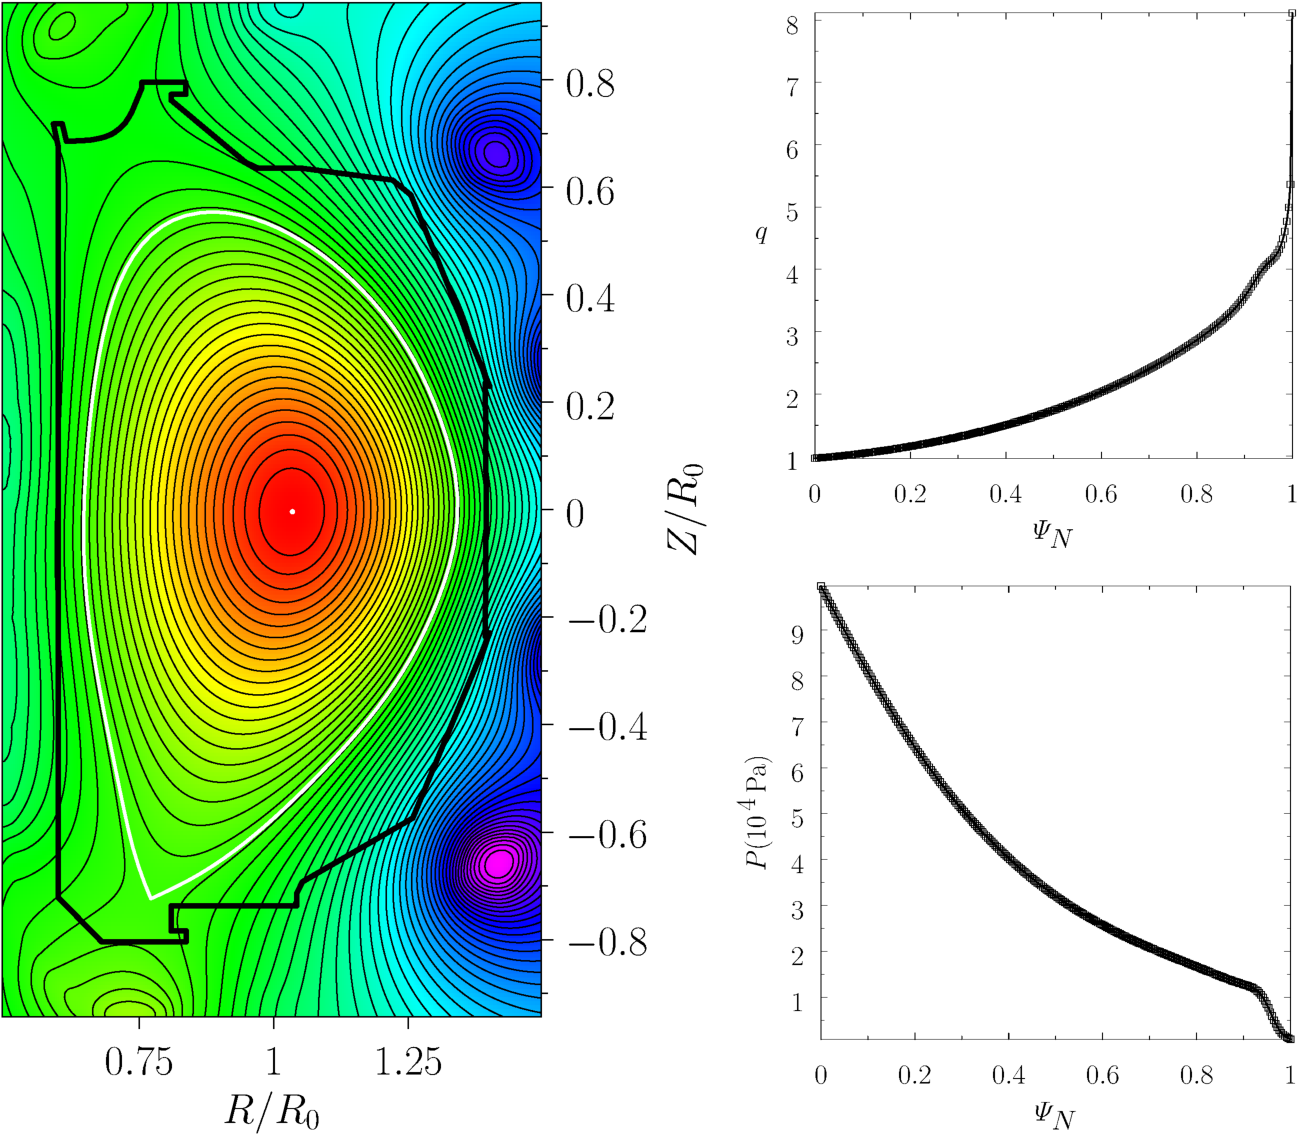
\includegraphics[height=5in]{fig2.pdf}
\caption{Left Panel: Contours of the equilibrium poloidal
magnetic flux in   DIII-D discharge \#145380 at time $t=2500$ ms. The scale major radius is $R_0=1.70\,{\rm m}$. The white dot indicates the magnetic axis, the white curve indicates the
last closed magnetic flux-surface, and the thick black line indicates the limiter. 
Upper-Right Panel: Safety-factor profile in DIII-D discharge \#145380 at time $t=2500$ ms. Lower-Right Panel:  Total plasma pressure profile in DIII-D discharge \#145380 at time $t=2500$ ms. } \label{fig2}
\end{figure}

\begin{figure}
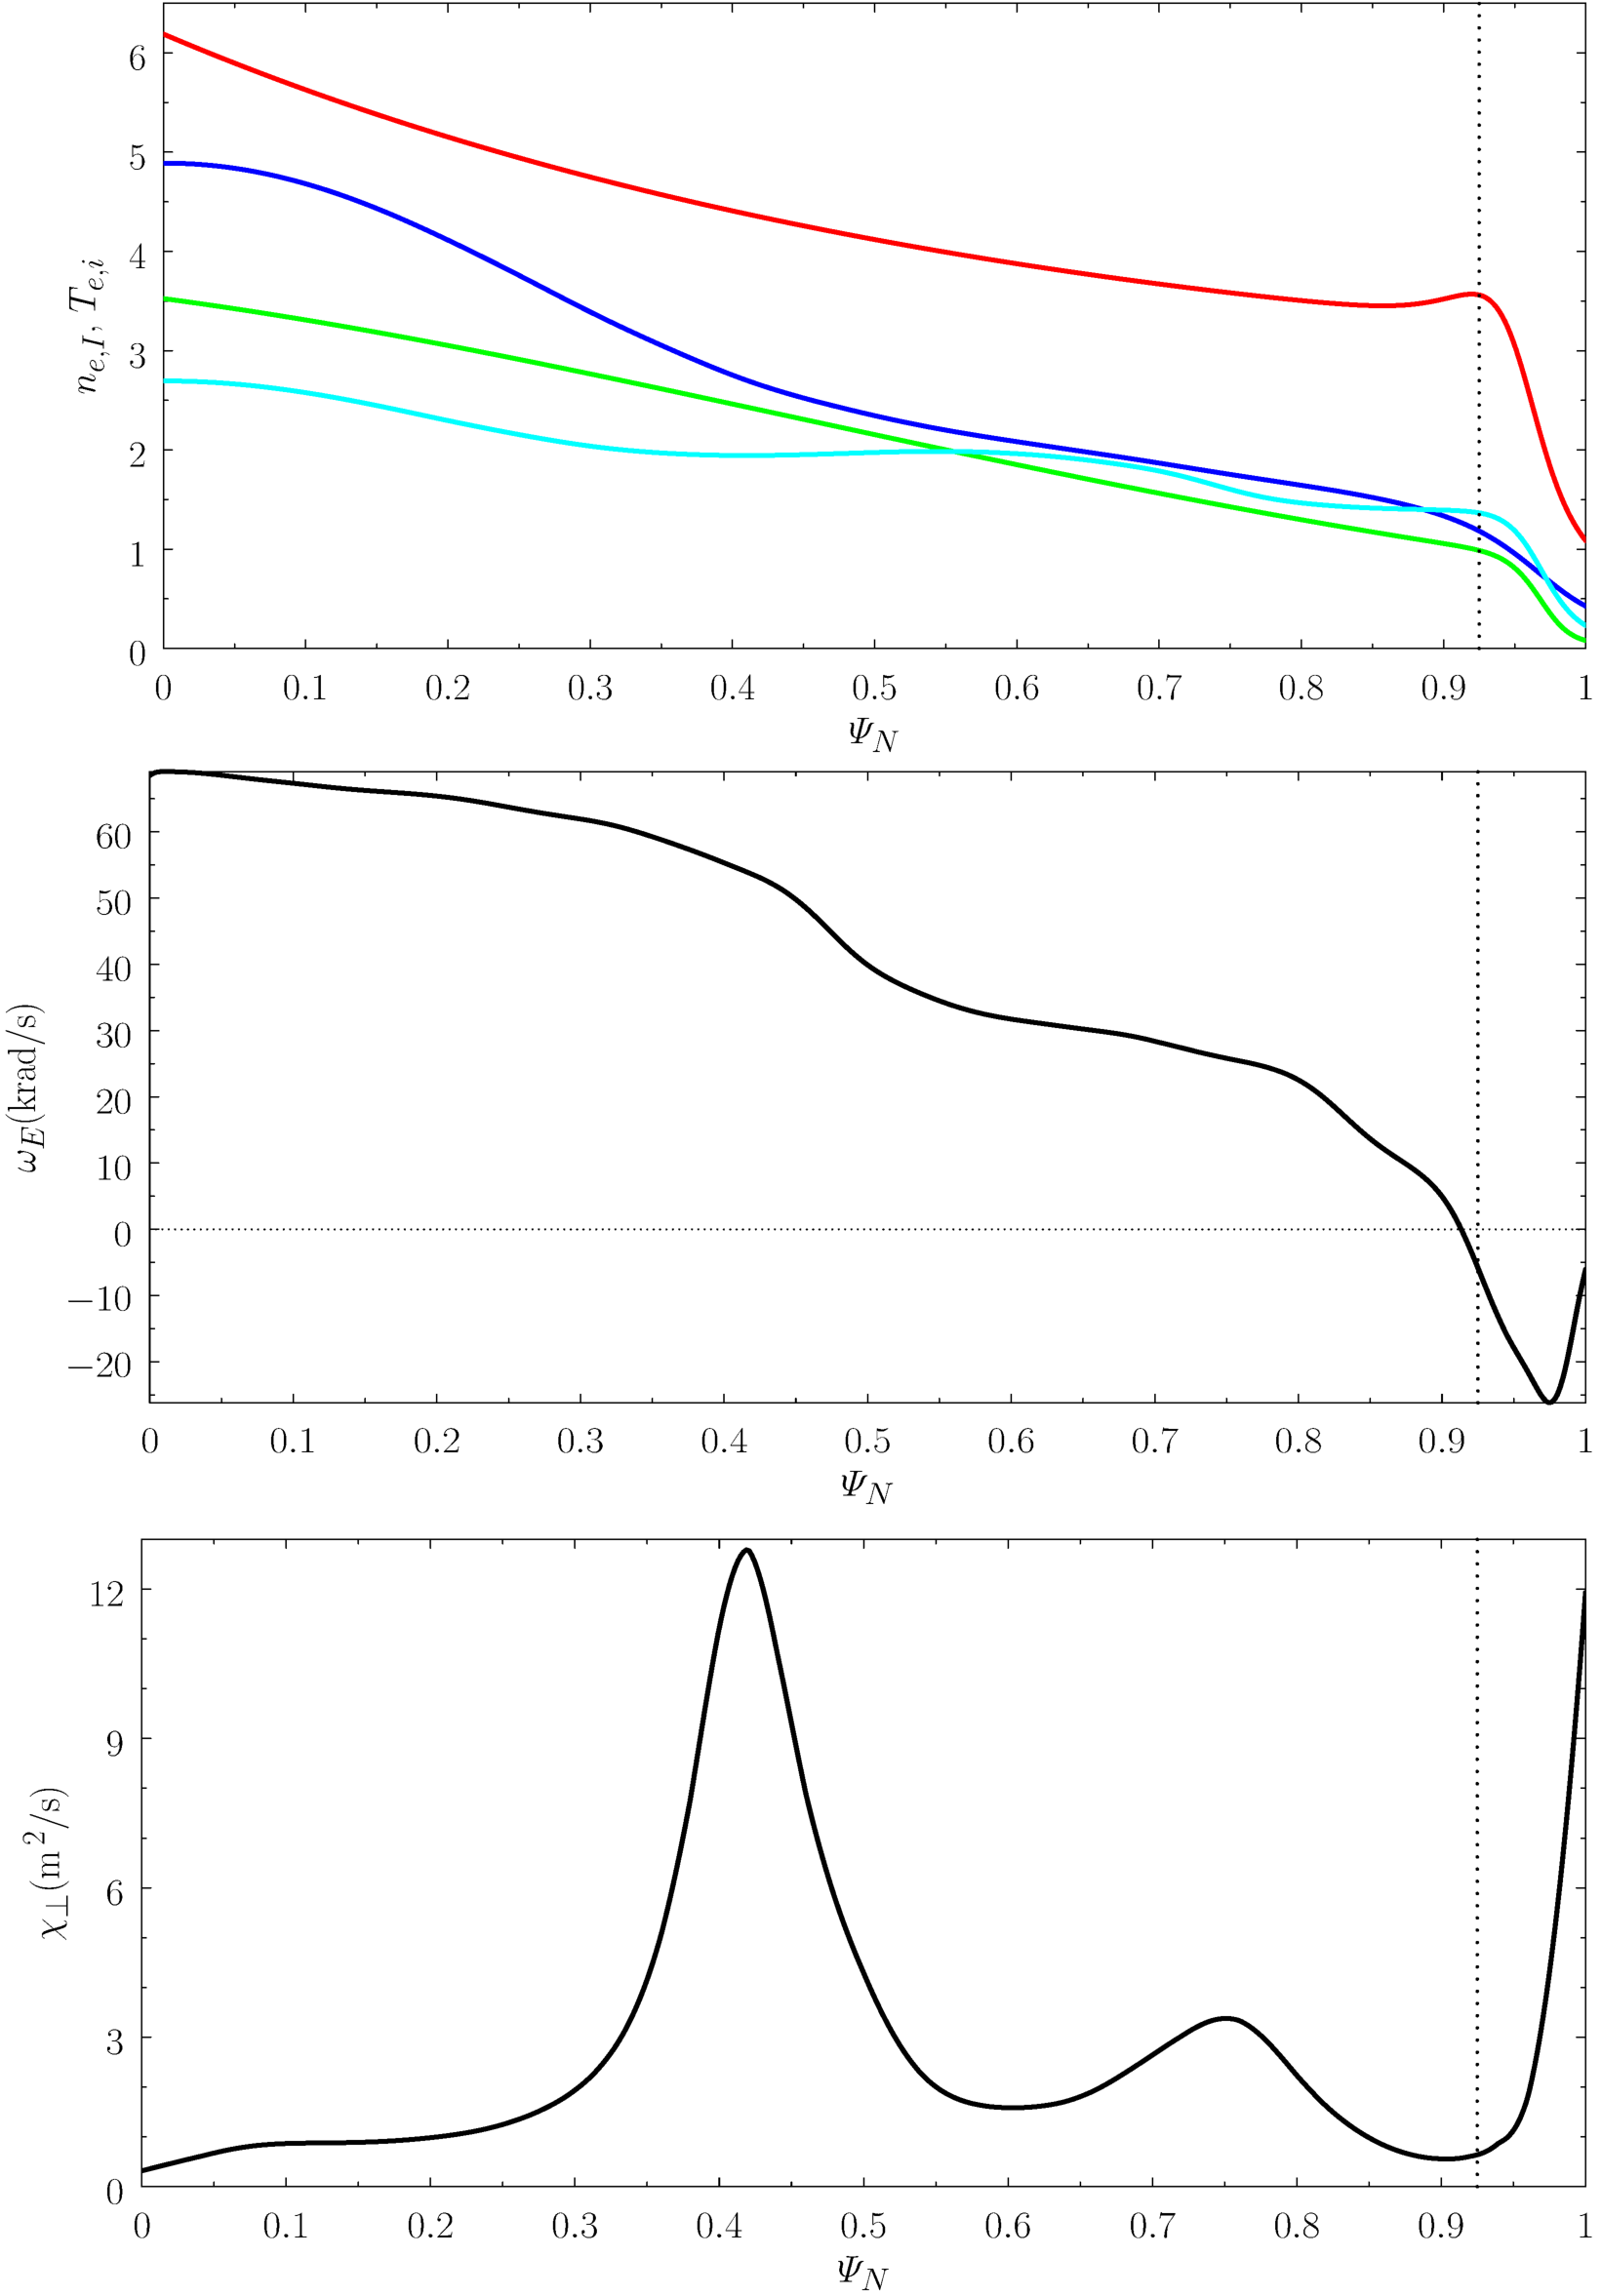
\includegraphics[height=7in]{fig3.pdf}
\caption{Top Panel: The red, green, blue, and cyan curves show the electron number density ($10^{19}\,{\rm m}^{-3}$),
electron temperature (keV), (thermal) ion temperature (keV), and
 C-VI ion number density  ($10^{18}\,{\rm m}^{-3}$)  profiles, respectively,  in  DIII-D discharge \#145380 at time $t=2500$ ms. Middle Panel:  
 ${\bf E}\times {\bf B}$ frequency profile in  DIII-D discharge \#145380 at time $t=2500$. Bottom Panel: The red, green, and blue curves show
 the perpendicular momentum, energy, and particle diffusivity profiles, respectively, 
 in  DIII-D discharge \#145380 at time $t=2500$ ms.
The   common vertical dotted lines indicate the location of the top
of the pedestal, ${\mit\Psi}_N=0.925$. In all cases, the thickness of the curves indicate the uncertainties in the measurements.} \label{fig3}
\end{figure}

\begin{figure}
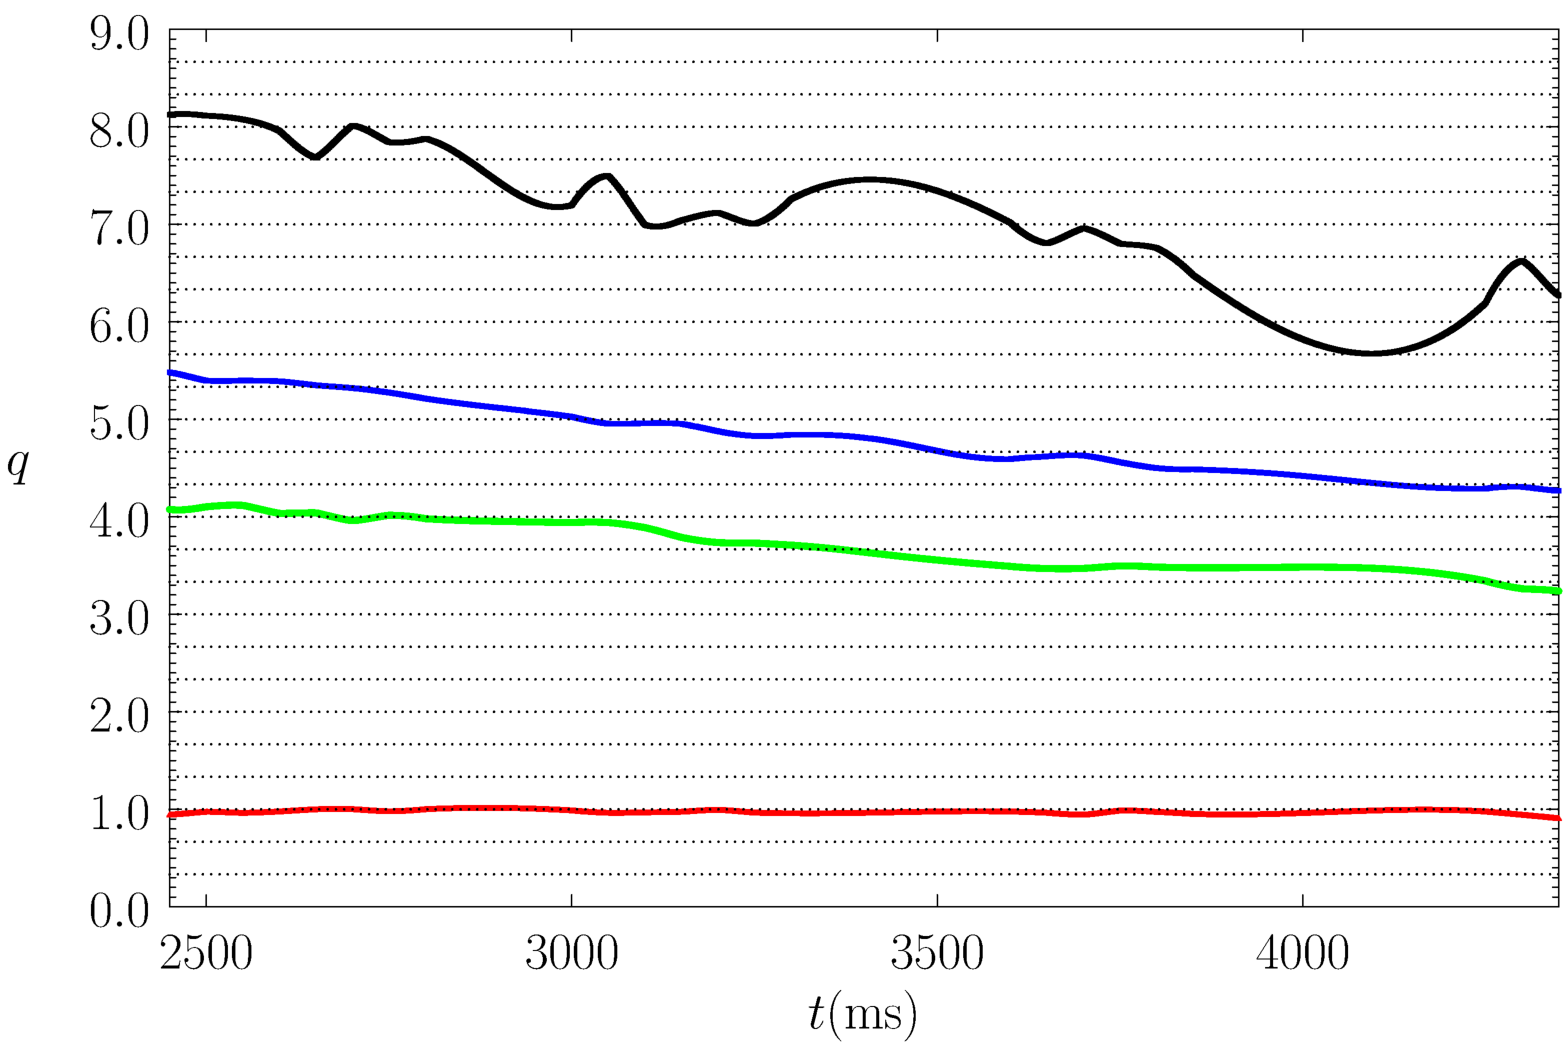
\includegraphics[height=4in]{fig4.pdf}
\caption{Safety-factors as functions of time in  DIII-D discharge \#145380. The red, green, blue, and black curves show the safety-factors
at the magnetic axis (${\mit\Psi}_N=0.00$),
the $95\%$ flux surface (${\mit\Psi}_N=0.950$), the
effective plasma boundary for the GPEC and EPEC calculations
(${\mit\Psi}_N=0.997$), and the true plasma boundary (${\mit\Psi}_N=1.00$), respectively. The yellow vertical bands indicate the ELM-suppression/mitigation windows. 
The horizontal dotted lines indicate the safety-factors at the various $n=3$ rational surfaces.} \label{fig4}
\end{figure}

\begin{figure}
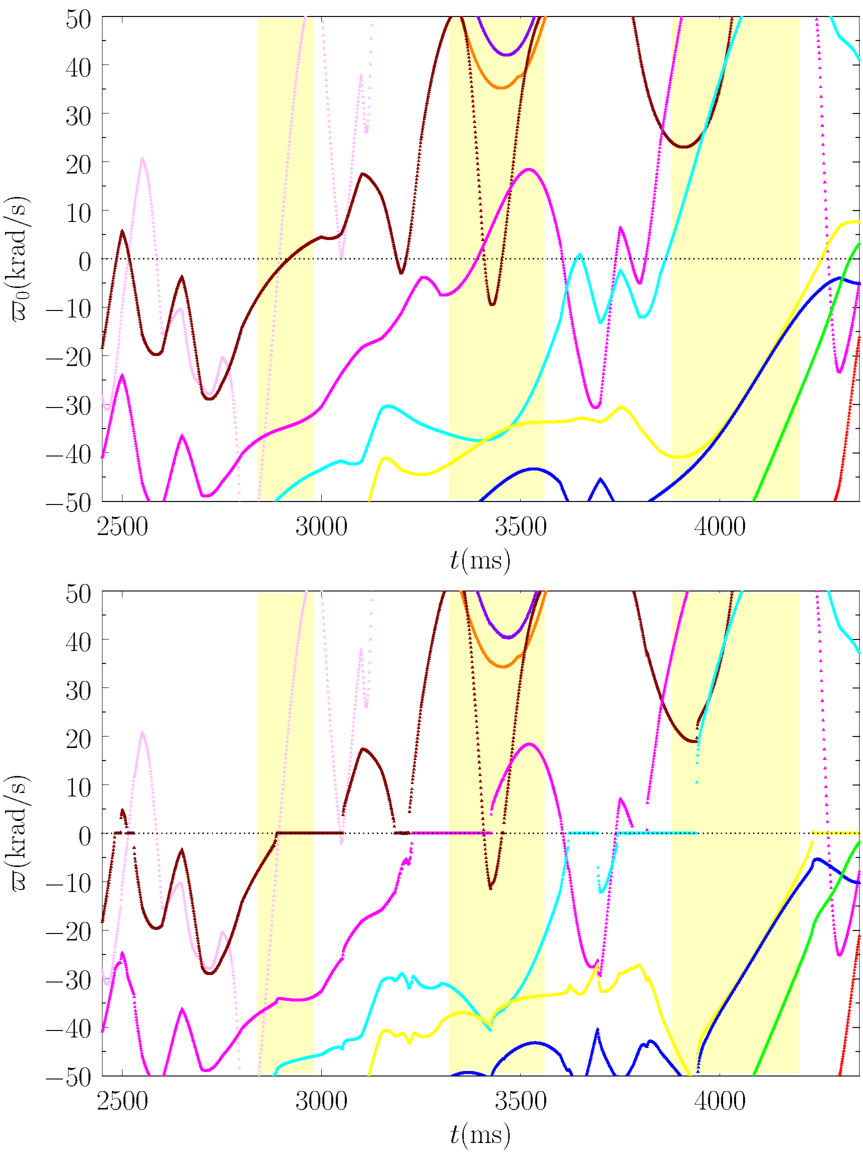
\includegraphics[height=6in]{fig5.pdf}
\caption{Top Panel: $n=3$ natural frequencies, in absence of RMP, as functions of the least-squares linear fit to $q_{95}$ versus time
in   DIII-D discharge \#145380, assuming that the natural frequency is determined by nonlinear island physics.
Bottom Panel:  $n=3$ natural frequencies, in presence of RMP, as functions of time
in   DIII-D discharge \#145380, assuming that the natural frequency is determined by nonlinear island physics. The red, green, blue, yellow, cyan, magenta, brown, pink,
purple, and orange  curves correspond to $m=5$, 6, 7, 8, 9, 10, 11, 12, 13, and 14, respectively. The yellow vertical bands indicate the ELM-suppression windows.} \label{fig5}
\end{figure}

\begin{figure}
\includegraphics[height=6in]{fig6.pdf}
\caption{Top Panel: Full  $n=3$ vacuum island widths as functions of the least-squares linear fit to $q_{95}$ versus time 
in   DIII-D discharge \#145380.
Bottom Panel:  Full $n=3$ island widths as functions of time
in   DIII-D discharge \#145380, assuming that the natural frequency is determined by nonlinear island physics. The blue, yellow, cyan, magenta, brown, pink,
purple, and orange  areas correspond to $m=7$, 8, 9, 10, 11, 12, 13, and 14, respectively. The yellow vertical bands indicate the ELM-suppression/mitigation windows. 
The horizontal dotted lines indicate the top of the pedestal, ${\mit\Psi}_N=0.925$.} \label{fig6}
\end{figure}

\begin{figure}
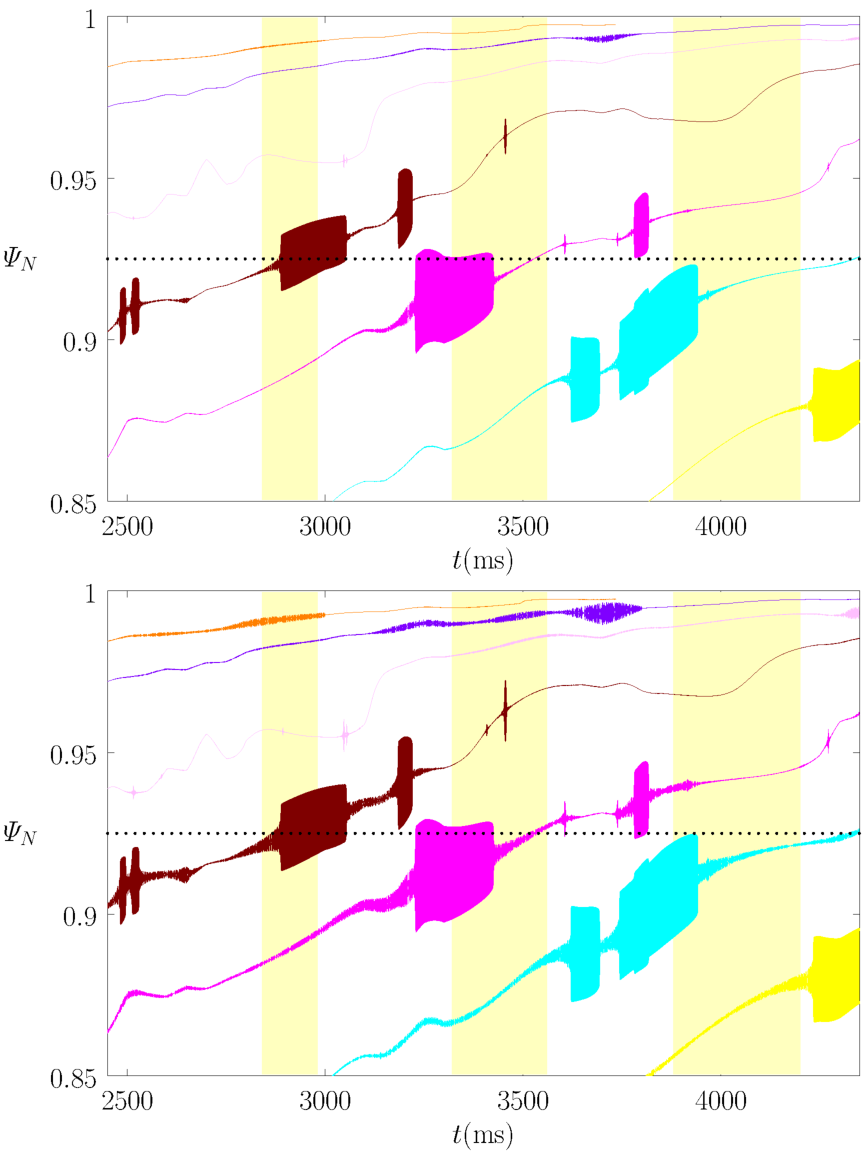
\includegraphics[height=6in]{fig7.pdf}
\caption{Top Panel: Density flattening widths associated with induced $n=3$ magnetic island  chains as functions of the least-squares linear fit to $q_{95}$ versus time
in   DIII-D discharge \#145380, assuming that the natural frequency is determined by nonlinear island physics.
Bottom Panel:  Electron temperature flattening widths associated with induced $n=3$ magnetic island chains as functions of time
in   DIII-D discharge \#145380, assuming that the natural frequency is determined by nonlinear island physics. The blue, yellow, cyan, magenta, brown, pink,
purple, and orange  areas correspond to $m=7$, 8, 9, 10, 11, 12, 13, and 14, respectively. The yellow vertical bands indicate the ELM-suppression/mitigation windows. 
The horizontal dotted lines indicate the top of the pedestal, ${\mit\Psi}_N=0.925$.} \label{fig7}
\end{figure}

\begin{figure}
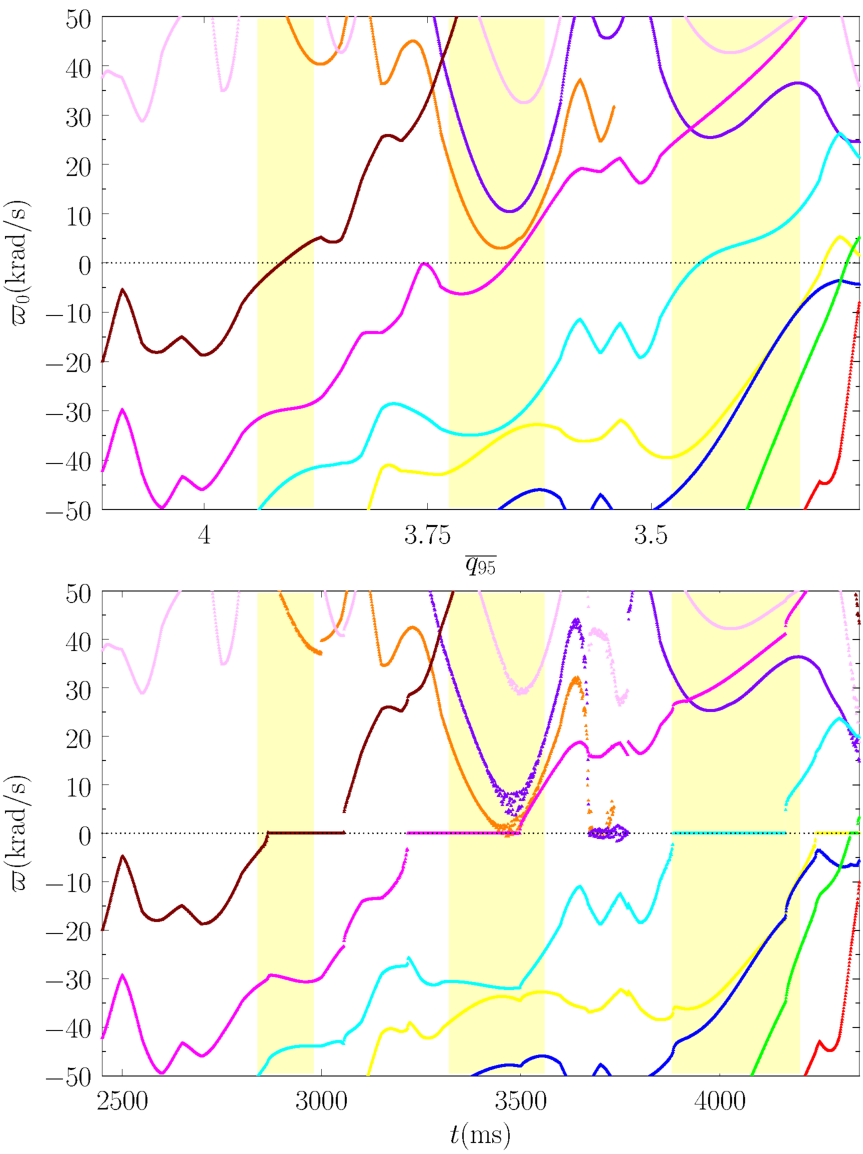
\includegraphics[height=6in]{fig8.pdf}
\caption{Top Panel: $n=3$ natural frequencies, in absence of RMP, as functions of the least-squares linear fit to $q_{95}$ versus time
in   DIII-D discharge \#145380, assuming that the natural frequency is determined by the ${\bf E}\times {\bf B}$
frequency.
Bottom Panel:  $n=3$ natural frequencies, in presence of RMP, as functions of time
in   DIII-D discharge \#145380, assuming that the natural frequency is  determined by the ${\bf E}\times {\bf B}$
frequency. The red, green, blue, yellow, cyan, magenta, brown, pink,
purple, and orange  curves correspond to $m=5$, 6, 7, 8, 9, 10, 11, 12, 13, and 14, respectively. The yellow vertical bands indicate the ELM-suppression/mitigation windows.} \label{fig8}
\end{figure}

\begin{figure}
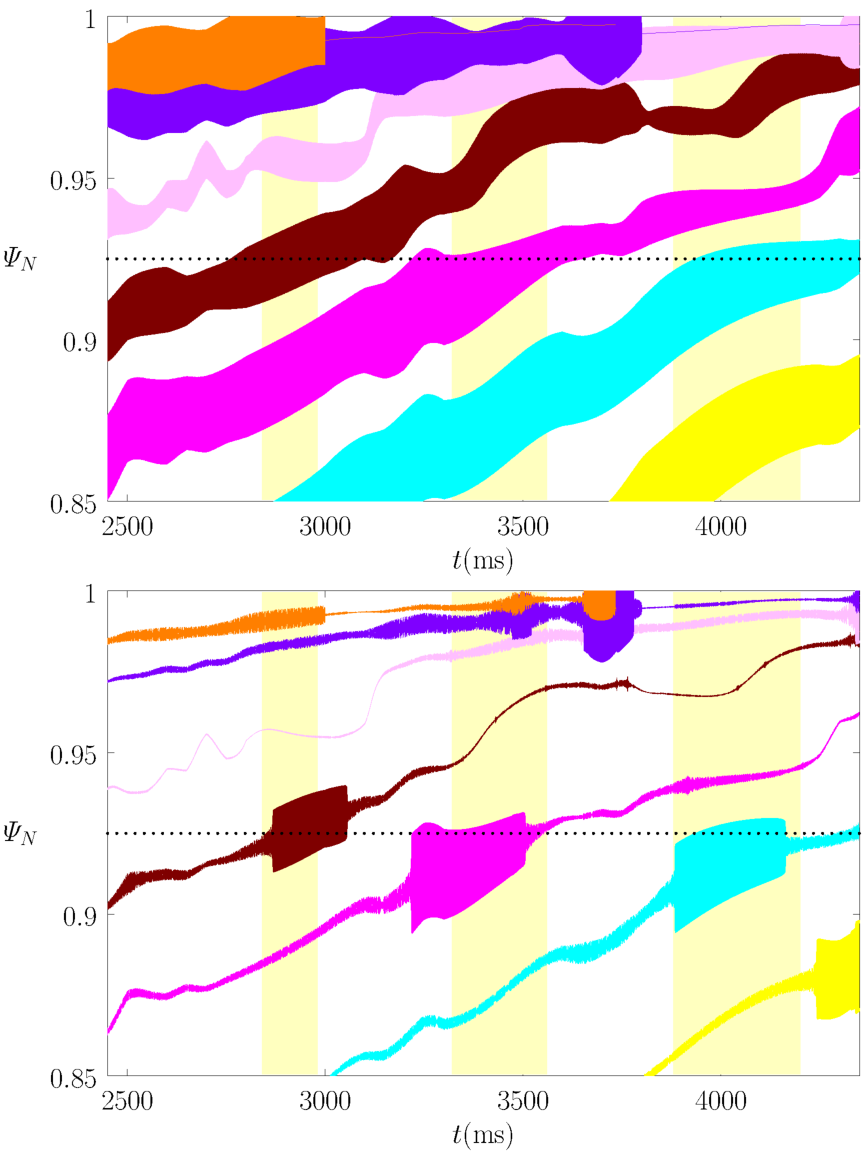
\includegraphics[height=6in]{fig9.pdf}
\caption{Top Panel: $n=3$ vacuum island widths as functions of the least-squares linear fit to $q_{95}$ versus time
in   DIII-D discharge \#145380.
Bottom Panel:  $n=3$ island widths as functions of time
in   DIII-D discharge \#145380, assuming that the natural frequency is  determined by the ${\bf E}\times {\bf B}$
frequency. The blue, yellow, cyan, magenta, brown, pink,
purple, and orange  areas correspond to $m=7$, 8, 9, 10, 11, 12, 13, and 14, respectively. The yellow vertical bands indicate the ELM-suppression/mitigation windows. 
The horizontal dotted lines indicate the top of the pedestal, ${\mit\Psi}_N=0.925$.} \label{fig9}
\end{figure}

\begin{figure}
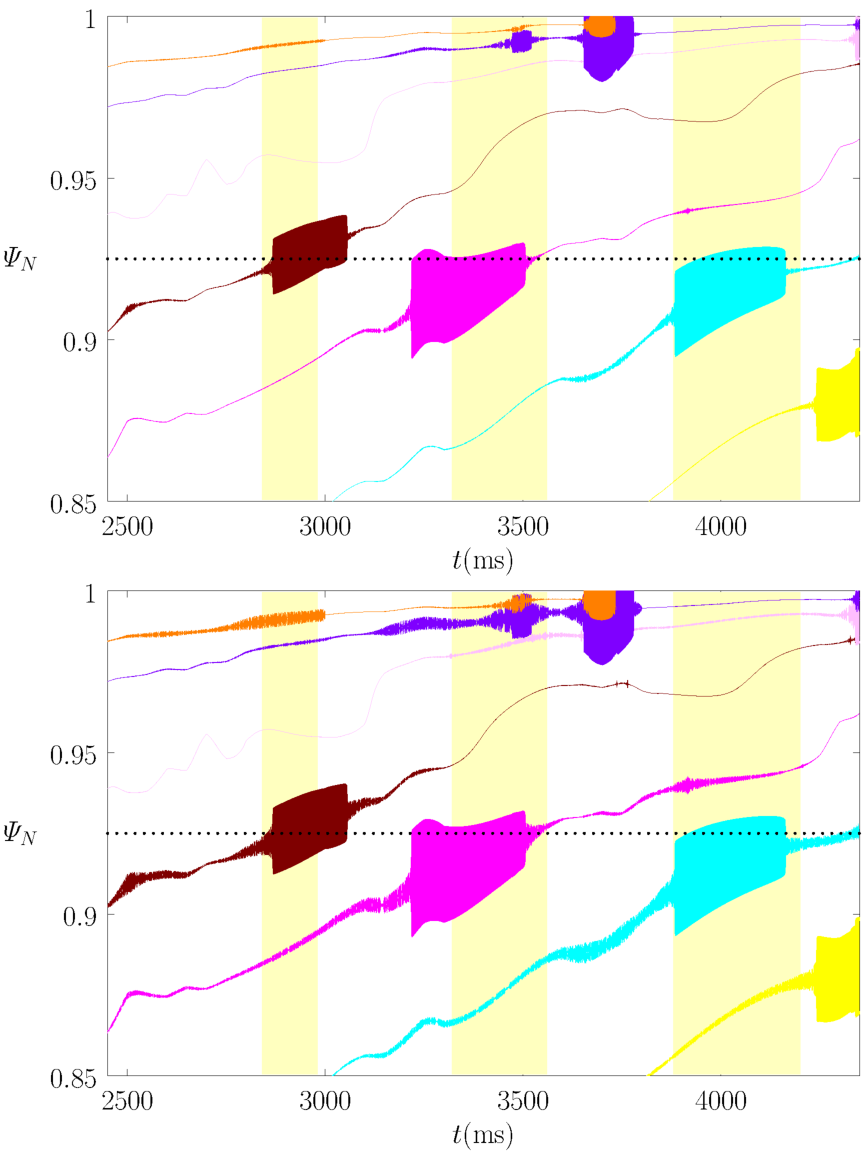
\includegraphics[height=6in]{fig10.pdf}
\caption{Top Panel: Density flattening widths associated with induced $n=3$ magnetic island  chains as functions of the least-squares linear fit to $q_{95}$ versus time
in   DIII-D discharge \#145380, assuming that the natural frequency is  determined by the ${\bf E}\times {\bf B}$
frequency.
Bottom Panel:  Electron temperature flattening widths associated with induced $n=3$ magnetic island chains as functions of time
in   DIII-D discharge \#145380, assuming that the natural frequency is determined by the ${\bf E}\times {\bf B}$
frequency. The blue, yellow, cyan, magenta, brown, pink,
purple, and orange  areas correspond to $m=7$, 8, 9, 10, 11, 12, 13, and 14, respectively. The yellow vertical bands indicate the ELM-suppression/mitigation windows. 
The horizontal dotted lines indicate the top of the pedestal, ${\mit\Psi}_N=0.925$.} \label{fig10}
\end{figure}

\begin{figure}
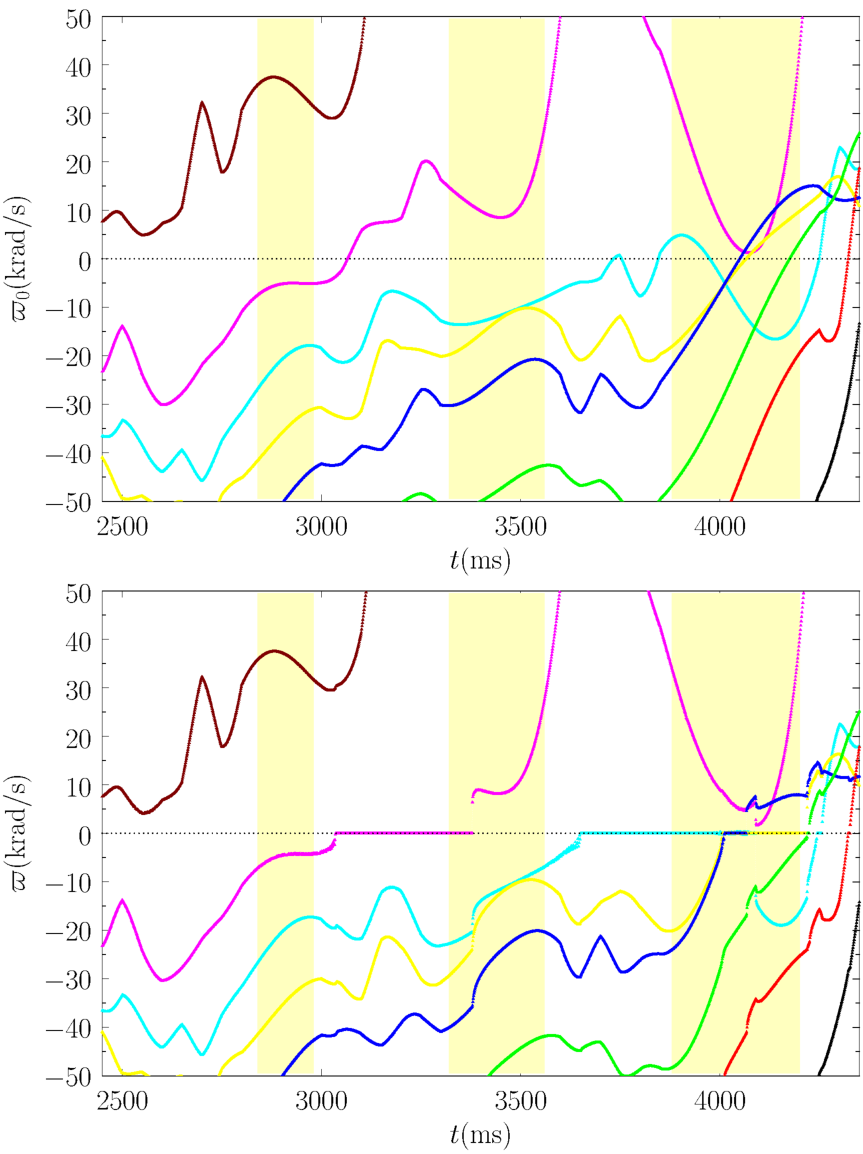
\includegraphics[height=6in]{fig11.pdf}
\caption{Top Panel: $n=3$ natural frequencies, in absence of RMP, as functions of the least-squares linear fit to $q_{95}$ versus time
in   DIII-D discharge \#145380, assuming that the natural frequency is determined by linear layer physics.
Bottom Panel:  $n=3$ natural frequencies, in presence of RMP, as functions of time
in   DIII-D discharge \#145380, assuming that the natural frequency is determined by linear layer physics. The black, red, green, blue, yellow, cyan, magenta,  brown, 
purple, and orange curves correspond to $m=4$, 5, 6, 7, 8, 9, 10,  11, 13, and 14, respectively. The yellow vertical bands indicate the ELM-suppression/mitigation windows.} \label{fig11}
\end{figure}

\begin{figure}
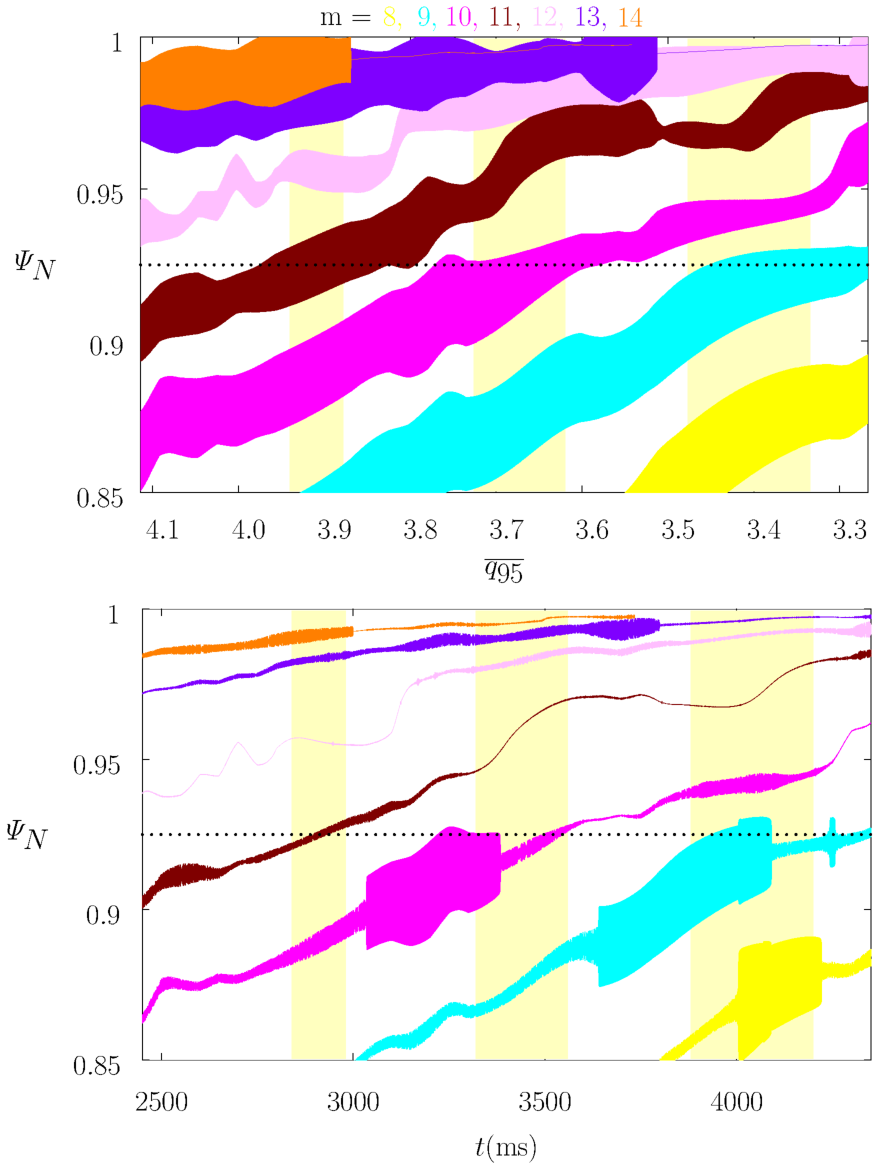
\includegraphics[height=6in]{fig12.pdf}
\caption{Top Panel: $n=3$ vacuum island widths as functions of the least-squares linear fit to $q_{95}$ versus time
in   DIII-D discharge \#145380.
Bottom Panel:  $n=3$ island widths as functions of time
in   DIII-D discharge \#145380, assuming that the natural frequency is determined by linear layer physics. The blue, yellow, cyan, magenta, brown, pink,
purple, and orange  areas correspond to $m=7$, 8, 9, 10, 11, 12, 13, and 14, respectively. The yellow vertical bands indicate the ELM-suppression/mitigation windows. 
The horizontal dotted lines indicate the top of the pedestal, ${\mit\Psi}_N=0.925$.} \label{fig12}
\end{figure}

\begin{figure}
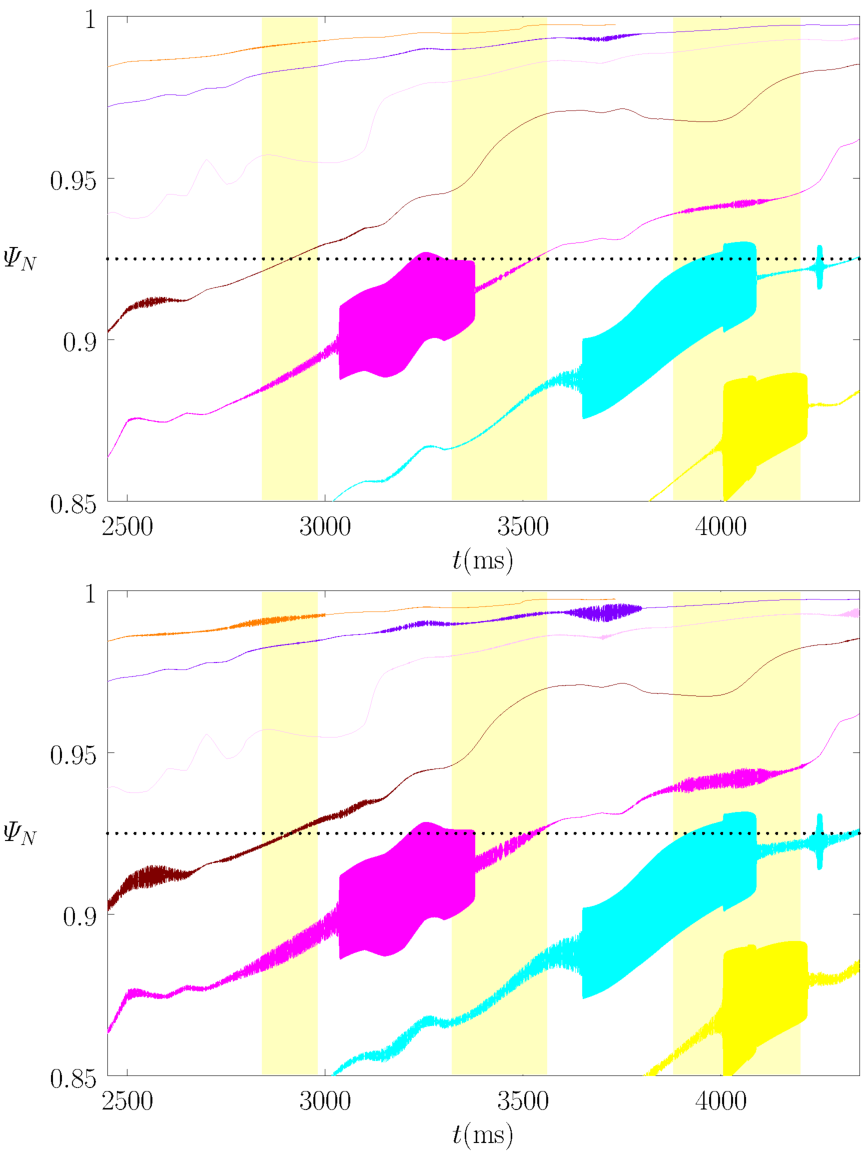
\includegraphics[height=6in]{fig13.pdf}
\caption{Top Panel: Density flattening widths associated with induced $n=3$ magnetic island  chains as functions of the least-squares linear fit to $q_{95}$ versus time
in   DIII-D discharge \#145380, assuming that the natural frequency is determined by linear layer physics.
Bottom Panel:  Electron temperature flattening widths associated with induced $n=3$ magnetic island chains as functions of time
in   DIII-D discharge \#145380, assuming that the natural frequency is determined by linear layer physics. The blue, yellow, cyan, magenta, brown, pink,
purple, and orange  areas correspond to $m=7$, 8, 9, 10, 11, 12, 13, and 14, respectively. The yellow vertical bands indicate the ELM-suppression/mitigation windows. 
The horizontal dotted lines indicate  the top of the pedestal, ${\mit\Psi}_N=0.925$.} \label{fig13}
\end{figure}

\begin{figure}
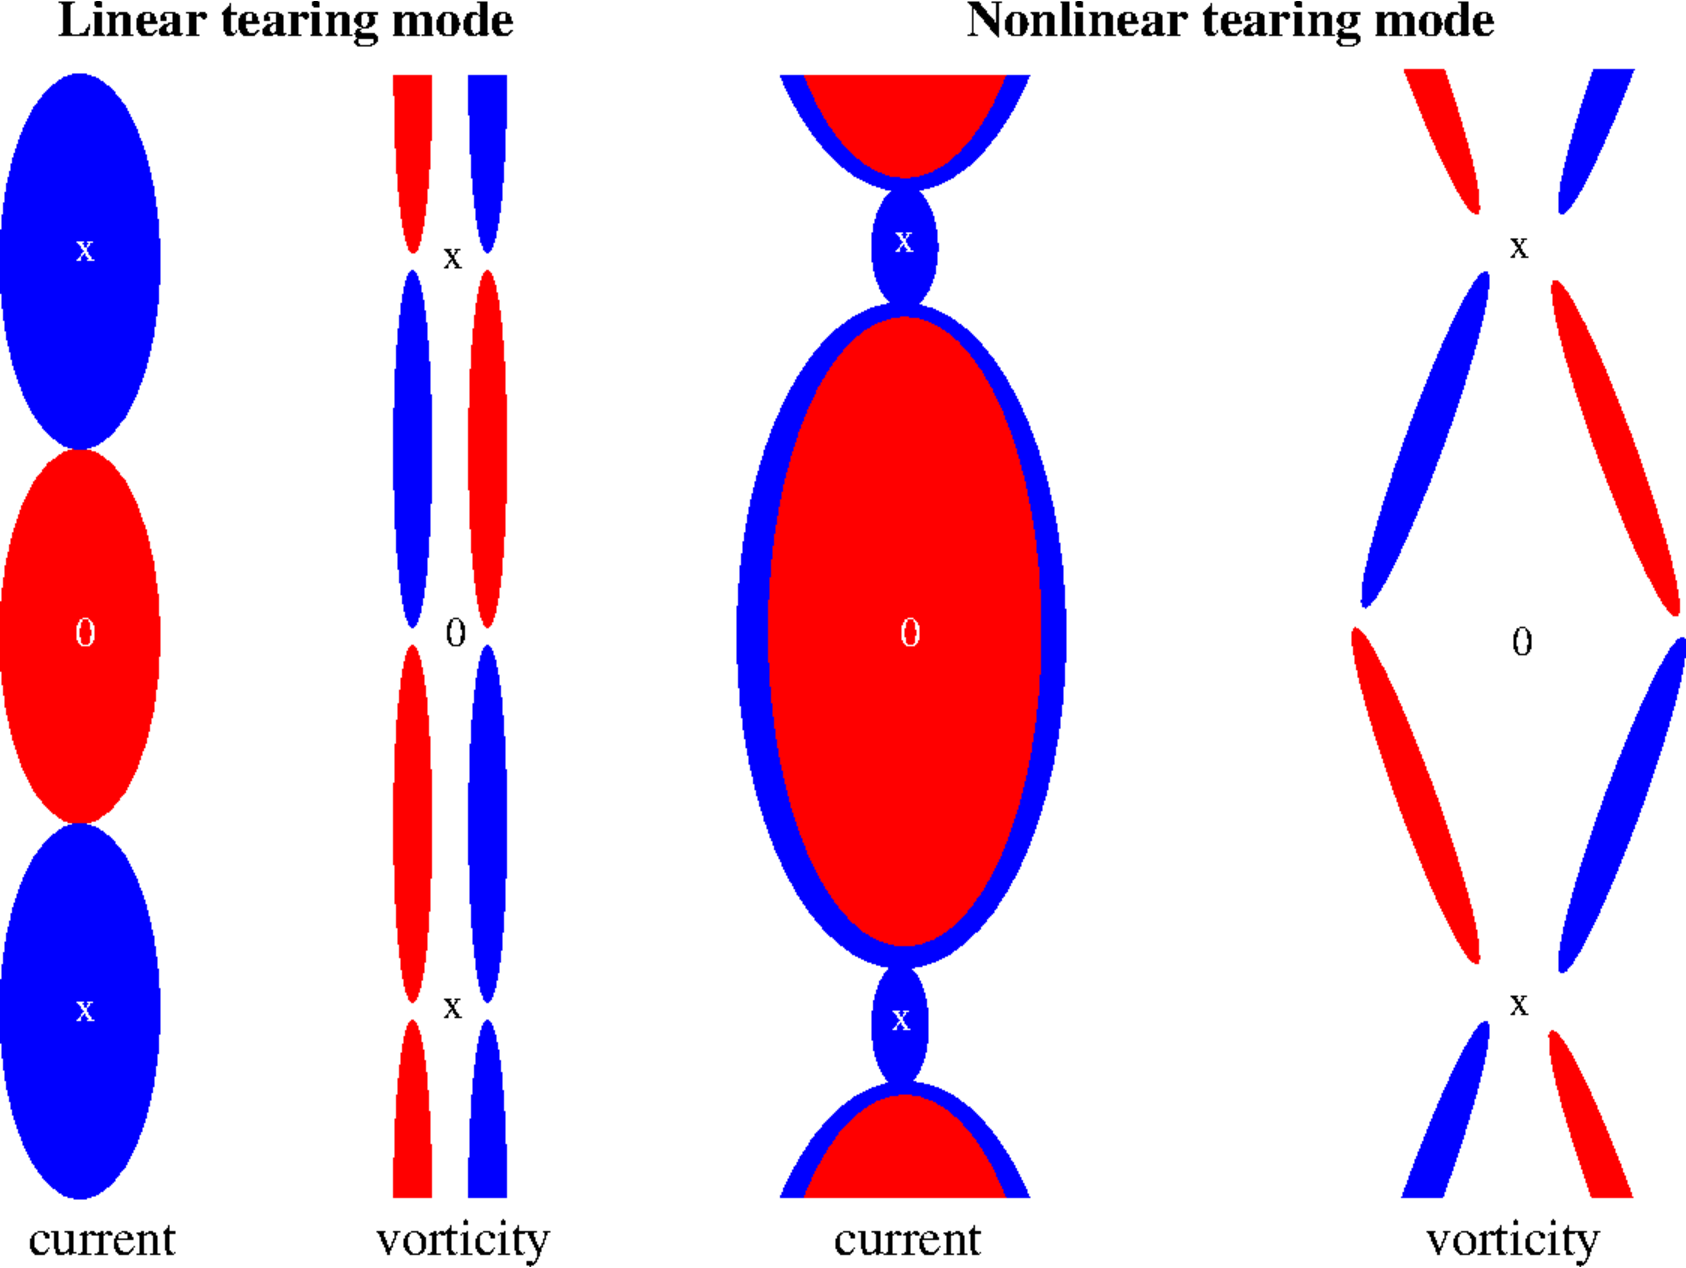
\includegraphics[height=4in]{fig14.pdf}
\caption{Schematic diagram showing the perturbed plasma current and vorticity patterns around the magnetic X- and O-points of a linear and a nonlinear tearing mode. 
The horizontal axis measures radial distance from the rational
surface, whereas the vertical axis measures distance along equilibrium magnetic field-lines. Red and blue
correspond to positive and negative current/vorticity values, respectively. (See Figs.~7 and 10 in 
Ref.~\onlinecite{rffig}.)}\label{fig14}
\end{figure}

\end{document}

